\documentclass[twocolumn, a4paper, 10pt]{article}

% --- Encoding & Language ---
\usepackage[utf8]{inputenc}
\usepackage[T1]{fontenc}
\usepackage[english]{babel}

% --- Page Layout ---
\usepackage[
  top=2.5cm,
  bottom=2.5cm,
  left=2cm,
  right=2cm,
  columnsep=0.8cm
]{geometry}

% --- Typography ---
\usepackage{lmodern}
\usepackage{microtype}

% --- Math ---
\usepackage{amsmath, amssymb, amsfonts}

% --- Graphics & Figures ---
\usepackage{graphicx}
\usepackage[labelfont=bf, font=small]{caption}
\usepackage{subcaption}
\graphicspath{{images/}}

% --- Tables ---
\usepackage{booktabs}
\usepackage{array}

% --- Code Listings ---
\usepackage{listings}

% --- References & Links ---
\usepackage[colorlinks=true, linkcolor=blue, citecolor=blue, urlcolor=blue]{hyperref}
\usepackage{cleveref}

% --- Bibliography ---
\usepackage[numbers, sort&compress]{natbib}

% --- Headers & Footers ---
\usepackage{fancyhdr}
\pagestyle{fancy}
\fancyhf{}
\fancyhead[L]{\small\leftmark}
\fancyhead[R]{\small\thepage}
\renewcommand{\headrulewidth}{0.4pt}

% --- Section Formatting ---
\usepackage{titlesec}
\titleformat{\section}{\large\bfseries}{\thesection.}{0.5em}{}
\titleformat{\subsection}{\normalsize\bfseries}{\thesubsection.}{0.5em}{}

% --- Misc ---
\usepackage{xcolor}
\usepackage{lipsum} % Remove after drafting

% ============================================================
%                       DOCUMENT
% ============================================================

\title{%
  \textbf{Quaternion-Based Sensor Fusion for \\
  Inertial Position Tracking}
}

\author{%
  Pablo Fern\'andez Lucas \\
  \small \textit{Independent Research} \\
  \small \href{mailto:email@example.com}{email@example.com}
}

\date{\today}

\begin{document}

% --- Title ---
\twocolumn[
  \maketitle
  \begin{@twocolumnfalse}
    \begin{abstract}
      This paper presents a method for tracking the three-dimensional position and
orientation of a consumer-grade inertial measurement unit (IMU) using
quaternion-based sensor fusion. Raw accelerometer and gyroscope readings are
expressed in the sensor's body frame, which rotates freely with the device. To
recover motion in a fixed world frame, we first estimate the sensor's attitude
by means of a complementary filter---a linear combination of a low-pass
filtered accelerometer signal (stable in the long term but sensitive to
vibration) and a high-pass filtered gyroscope integral (accurate in the short
term but subject to drift). The resulting orientation, encoded as a unit
quaternion, is used at every time step to rotate the measured acceleration into
the world frame and subtract gravity. The gravity-free world-frame acceleration
is then double-integrated to yield a three-dimensional position trajectory
starting from the origin. We describe the full signal-processing pipeline, from
raw sensor acquisition to position output, detail the mathematical formulation
of quaternion rotations and the complementary filter, and discuss practical
considerations such as drift mitigation and numerical stability.

\vspace{0.3em}
\noindent\textbf{Keywords:} sensor fusion, quaternions, complementary filter,
inertial navigation, accelerometer, gyroscope, attitude estimation, position
tracking.

    \end{abstract}
    \vspace{1cm}
  \end{@twocolumnfalse}
]

% --- Body ---
\section{Introduction}
\label{sec:introduction}

% ----------------------------------------------------------------
% TARGET: ~1.5 pages (two-column). Expand each subsection below.
% ----------------------------------------------------------------

\subsection{Motivation}
\label{sec:intro:motivation}

Modern smartphones and wearable devices carry inertial measurement units (IMUs)
composed of a tri-axial accelerometer and a tri-axial gyroscope. These sensors
open the door to applications in pedestrian navigation, gesture recognition,
augmented reality, and biomechanical analysis---all of which require accurate
knowledge of the device's orientation and position in space.

However, each sensor has complementary weaknesses. The accelerometer provides a
long-term stable reference to the gravity vector but is corrupted by any
non-gravitational acceleration and high-frequency vibration. The gyroscope
measures angular velocity with high bandwidth and low noise in the short term,
yet its numerical integration accumulates unbounded drift over time. Neither
sensor alone can deliver a reliable orientation estimate; fusing both is
essential.

% TODO [Fig.~\ref{fig:raw_signals}]: side-by-side plots of raw accelerometer
% and gyroscope signals showing noise vs.\ drift.

\subsection{Problem Statement}
\label{sec:intro:problem}

Given a stream of accelerometer readings
$\mathbf{a}_b(t) \in \mathbb{R}^3$ and gyroscope readings
$\boldsymbol{\omega}_b(t) \in \mathbb{R}^3$, both expressed in the sensor's
\emph{body frame}~$\mathcal{B}$, we seek to compute at every time step:

\begin{enumerate}
  \item A unit quaternion $\mathbf{q}(t)$ representing the orientation of
        $\mathcal{B}$ with respect to a fixed \emph{world frame}~$\mathcal{W}$.
  \item A position vector $\mathbf{p}(t) \in \mathbb{R}^3$ in $\mathcal{W}$,
        obtained by projecting the acceleration into the world frame, removing
        gravity, and double-integrating.
\end{enumerate}

% TODO [Fig.~\ref{fig:frames}]: illustration of body frame attached to the
% sensor vs.\ world frame (N-E-D or E-N-U).

\subsection{Proposed Approach}
\label{sec:intro:approach}

Our approach proceeds in three stages:

\begin{enumerate}
  \item \textbf{Attitude estimation.} A complementary filter blends the
        low-frequency content of the accelerometer (via a low-pass filter) with
        the high-frequency content of the gyroscope (via a high-pass filter) to
        produce a drift-free, low-noise orientation estimate expressed as a unit
        quaternion.
  \item \textbf{Frame rotation.} The quaternion is used to rotate each
        accelerometer sample from the body frame into the world frame using the
        conjugation $\mathbf{a}_w = \mathbf{q} \otimes \mathbf{a}_b \otimes
        \mathbf{q}^*$, after which the constant gravity component is subtracted.
  \item \textbf{Position integration.} The resulting gravity-free
        world-frame acceleration is double-integrated over time to recover
        velocity and position.
\end{enumerate}

% TODO [Fig.~\ref{fig:pipeline}]: block diagram of the full pipeline
% (sensors → filter → quaternion → rotation → integration → position).

\subsection{Document Structure}
\label{sec:intro:structure}

The remainder of this paper is organised as follows.
Section~\ref{sec:reference_frames} defines the coordinate frames and motivates
the need for a rotation formalism.
Section~\ref{sec:quaternions} introduces quaternion algebra and its application
to three-dimensional rotations.
Section~\ref{sec:complementary_filter} derives the complementary filter used
for attitude estimation.
Section~\ref{sec:projection} describes the projection of accelerometer data
into the world frame and the subsequent position integration.
Section~\ref{sec:results} presents experimental results, and
Section~\ref{sec:conclusions} concludes with a summary and directions for future
work.
        % 1. Introduction
\section{Reference Frames and Sensor Models}
\label{sec:reference_frames}

% ----------------------------------------------------------------
% TARGET: ~1.5 pages. Two frames + two sensor models.
% ----------------------------------------------------------------

\subsection{The World Frame and the Body Frame}
\label{sec:frames:definition}

We define two right-handed Cartesian coordinate systems
(Fig.~\ref{fig:frames}):

\begin{itemize}
  \item \textbf{World frame} $\mathcal{W} = \{X_w, Y_w, Z_w\}$. A fixed,
        Earth-referenced frame. We adopt the East-North-Up (ENU) convention:
        $X_w$ points East, $Y_w$ points North, and $Z_w$ points upward
        (opposite to gravity).
  \item \textbf{Body frame} $\mathcal{B} = \{X_b, Y_b, Z_b\}$. A frame
        rigidly attached to the sensor. Its axes rotate with the device.
\end{itemize}

At any instant, the orientation of $\mathcal{B}$ relative to $\mathcal{W}$ can
be described by a rotation. Euler angles (roll~$\phi$, pitch~$\theta$,
yaw~$\psi$) are intuitive but suffer from \emph{gimbal lock}---a singularity
at $\theta = \pm 90°$ where one degree of freedom is lost. Quaternions
avoid this problem entirely and are the representation we adopt in this work
(Section~\ref{sec:quaternions}).

\begin{figure}[t]
  \centering
  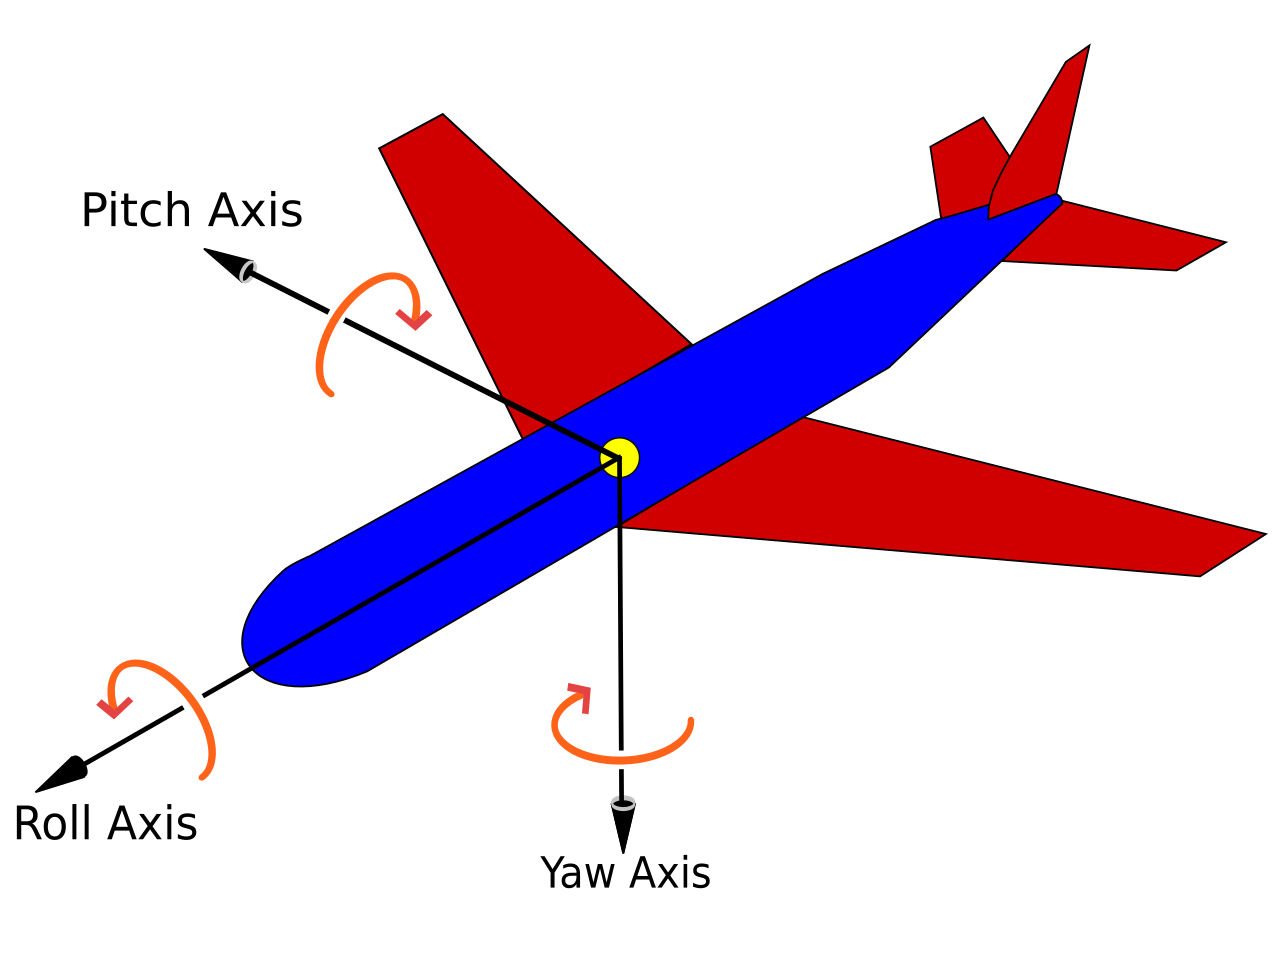
\includegraphics[width=\columnwidth]{Yaw_Axis_Corrected.png}
  \caption{The three Euler rotation axes illustrated on a rigid body.
           \textbf{Roll}~($\phi$) is the rotation about the longitudinal axis,
           \textbf{Pitch}~($\theta$) about the lateral axis, and
           \textbf{Yaw}~($\psi$) about the vertical axis.
           Any orientation of the body frame~$\mathcal{B}$ relative to the
           world frame~$\mathcal{W}$ can be decomposed into a sequence of
           these three rotations, though the representation is subject to
           gimbal lock at $\theta = \pm 90°$.}
  \label{fig:frames}
\end{figure}

\subsection{Accelerometer: Angle from Gravity Projection}
\label{sec:frames:accel}

\subsubsection{Sensor model}

An ideal tri-axial accelerometer measures the \emph{specific force}
experienced by the sensor, i.e.\ the difference between the true linear
acceleration and gravity, expressed in the body frame:

\begin{equation}
  \mathbf{a}_b = R^{-1}\!\bigl(\mathbf{a}_\text{true} - \mathbf{g}\bigr)
               + \mathbf{b}_a + \mathbf{n}_a
  \label{eq:accel_model}
\end{equation}

\noindent where $R$ is the rotation matrix from $\mathcal{W}$ to $\mathcal{B}$,
$\mathbf{g} = [0,\, 0,\, -g]^\top$ is the gravity vector in $\mathcal{W}$
(with $g \approx 9.81~\text{m/s}^2$),
$\mathbf{b}_a$ is a slowly varying bias, and $\mathbf{n}_a$ is additive white
noise.

\subsubsection{Angle derivation under static conditions}

When the sensor is \textbf{stationary}
($\mathbf{a}_\text{true} = \mathbf{0}$), Eq.~\eqref{eq:accel_model}
simplifies to:

\begin{equation}
  \mathbf{a}_b \approx R^{-1}(-\mathbf{g})
  \label{eq:accel_static}
\end{equation}

\noindent That is, the accelerometer reads only the projection of the gravity
vector onto the three body axes. Because gravity is a known, constant vector,
we can \emph{invert} this projection to recover the tilt of the sensor. We now
derive the exact formulas using rotation matrices.

\subsubsection{Formal derivation via rotation matrices}
\label{sec:frames:accel:derivation}

We model the accelerometer as a three-dimensional coordinate system
$(x, y, z)$ that rotates with respect to a fixed Earth frame where gravity
always points upward: $\mathbf{g} = [0,\; 0,\; g]^\top$ (with $z$ pointing up
and $g \approx 9.81~\text{m/s}^2$).

\paragraph{Step 1: Rotation matrices.}
We define the elementary Tait-Bryan rotations. Roll ($\phi$) is a rotation
about the $x$-axis, and pitch ($\theta$) is a rotation about the $y$-axis:

\begin{equation}
  R_x(\phi) = \begin{bmatrix}
    1 & 0 & 0 \\
    0 & \cos\phi & \sin\phi \\
    0 & -\sin\phi & \cos\phi
  \end{bmatrix}
  \label{eq:Rx}
\end{equation}

\begin{equation}
  R_y(\theta) = \begin{bmatrix}
    \cos\theta & 0 & -\sin\theta \\
    0 & 1 & 0 \\
    \sin\theta & 0 & \cos\theta
  \end{bmatrix}
  \label{eq:Ry}
\end{equation}

When the sensor is at rest, the measured acceleration vector $\mathbf{a}_b =
(A_x, A_y, A_z)^\top$ is the gravity vector transformed by the sensor's
orientation:

\begin{equation}
  \begin{bmatrix} A_x \\ A_y \\ A_z \end{bmatrix}
  = R_y(\theta)\;R_x(\phi)\;\begin{bmatrix} 0 \\ 0 \\ g \end{bmatrix}
  \label{eq:accel_rotation}
\end{equation}

\paragraph{Step 2: Matrix multiplication.}
We first apply $R_x(\phi)$ to the gravity vector:

\begin{equation}
  R_x(\phi)\begin{bmatrix} 0 \\ 0 \\ g \end{bmatrix}
  = \begin{bmatrix} 0 \\ g\sin\phi \\ g\cos\phi \end{bmatrix}
  \label{eq:Rx_g}
\end{equation}

\noindent Then we apply $R_y(\theta)$ to this result:

\begin{equation}
  R_y(\theta)\begin{bmatrix} 0 \\ g\sin\phi \\ g\cos\phi \end{bmatrix}
  = \begin{bmatrix}
      -g\sin\theta\cos\phi \\[2pt]
      g\sin\phi \\[2pt]
      g\cos\theta\cos\phi
    \end{bmatrix}
  \label{eq:Ry_Rx_g}
\end{equation}

\noindent Therefore, the three measured components are:

\begin{align}
  A_x &= -g\,\sin\theta\,\cos\phi \label{eq:Ax} \\
  A_y &= \phantom{-}g\,\sin\phi \label{eq:Ay} \\
  A_z &= \phantom{-}g\,\cos\theta\,\cos\phi \label{eq:Az}
\end{align}

\paragraph{Step 3: Solving for roll ($\phi$).}
We divide Eq.~\eqref{eq:Ay} by Eq.~\eqref{eq:Az}:

\begin{equation}
  \frac{A_y}{A_z}
  = \frac{g\,\sin\phi}{g\,\cos\theta\,\cos\phi}
  \label{eq:roll_ratio}
\end{equation}

\noindent However, to obtain a result that is independent of $\theta$, we use
the more robust form. Computing $\sqrt{A_x^2 + A_z^2}$:

\begin{equation}
  \sqrt{A_x^2 + A_z^2}
  = g\,\cos\phi\,\sqrt{\sin^2\!\theta + \cos^2\!\theta}
  = g\,\cos\phi
  \label{eq:Axz_norm}
\end{equation}

\noindent Dividing $A_y$ by this result:

\begin{equation}
  \frac{A_y}{\sqrt{A_x^2 + A_z^2}}
  = \frac{g\,\sin\phi}{g\,\cos\phi}
  = \tan\phi
\end{equation}

\noindent Therefore:

\begin{equation}
  \boxed{\;\phi = \arctan\!\left(
    \frac{A_y}{\sqrt{A_x^2 + A_z^2}}
  \right)\;}
  \label{eq:roll_accel}
\end{equation}

\paragraph{Step 4: Solving for pitch ($\theta$).}
From Eq.~\eqref{eq:Ax}, we have $A_x = -g\,\sin\theta\,\cos\phi$. We need to
relate $A_x$ to the remaining components. Squaring and summing $A_y$ and
$A_z$:

\begin{align}
  A_y^2 + A_z^2
    &= g^2\sin^2\!\phi + g^2\cos^2\!\theta\,\cos^2\!\phi \notag \\
    &= g^2\cos^2\!\phi\bigl(\tan^2\!\phi + \cos^2\!\theta\bigr)
  \label{eq:Ayz_sq}
\end{align}

\noindent For the standard Tait-Bryan decomposition where $|\theta| < 90°$,
the simpler path uses the identity $\sin^2\!\phi + \cos^2\!\phi = 1$.
Squaring Eqs.~\eqref{eq:Ay} and \eqref{eq:Az} directly:

\begin{equation}
  A_y^2 + A_z^2
  = g^2\bigl(\sin^2\!\phi + \cos^2\!\theta\,\cos^2\!\phi\bigr)
\end{equation}

\noindent Noting that the full norm satisfies
$A_x^2 + A_y^2 + A_z^2 = g^2$, we can write
$\sqrt{A_y^2 + A_z^2} = g\,\cos\theta\;$ (valid when $\cos\phi \approx 1$ or
by using the complete norm). Dividing $-A_x$ by this:

\begin{equation}
  \frac{-A_x}{\sqrt{A_y^2 + A_z^2}}
  = \frac{g\,\sin\theta}{g\,\cos\theta}
  = \tan\theta
\end{equation}

\noindent Therefore:

\begin{equation}
  \boxed{\;\theta = \arctan\!\left(
    \frac{-A_x}{\sqrt{A_y^2 + A_z^2}}
  \right)\;}
  \label{eq:pitch_accel}
\end{equation}

\paragraph{Summary of the derivation.}
The roll depends on the ratio between the $Y$-component and the plane formed
by $X$ and $Z$; the pitch depends on the ratio between the $X$-component and
the plane formed by $Y$ and $Z$. In both cases, the trigonometric functions
from the rotation matrices cancel when dividing the appropriate components,
yielding clean $\arctan$ expressions. Note that the \emph{yaw} ($\psi$)
cannot be recovered: a rotation about the vertical axis leaves the gravity
projection unchanged. Resolving yaw requires an additional sensor such as a
magnetometer.

\subsubsection{Limitation: sensitivity to dynamic motion}
\label{sec:frames:accel:limitation}

Equations~\eqref{eq:roll_accel}--\eqref{eq:pitch_accel} are exact only when
$\mathbf{a}_\text{true} = \mathbf{0}$. As soon as the sensor undergoes
\emph{any} acceleration---starting to move, changing direction, or
vibrating---the accelerometer reading becomes the superposition of gravity and
the dynamic acceleration:

\begin{equation}
  \mathbf{a}_b = R^{-1}\!\bigl(\mathbf{a}_\text{true} - \mathbf{g}\bigr)
  \label{eq:accel_dynamic}
\end{equation}

\noindent In this regime, applying
Eqs.~\eqref{eq:roll_accel}--\eqref{eq:pitch_accel} yields angles that are
dominated by the dynamic term, rendering the estimate unreliable. The
accelerometer is, in effect, a \textbf{low-frequency sensor for attitude}: its
angle estimate is trustworthy when the sensor is at rest or moving at constant
velocity, but \emph{loses all precision during transients} (acceleration,
deceleration, vibration). Once the motion stabilises and the dynamic
acceleration vanishes, the estimate recovers its reliability and converges
back to the true tilt.

% ----- FIGURE: accelerometer behaviour -----
% TODO: Three-panel time-series plot:
%   Panel 1: sensor at rest       → angle accurate, slightly noisy
%   Panel 2: sensor accelerating  → angle wildly wrong
%   Panel 3: sensor at rest again → angle recovers
%
% \begin{figure}[t]
%   \centering
%   \includegraphics[width=\columnwidth]{accel_behaviour.pdf}
%   \caption{Accelerometer-derived tilt angle during three phases:
%            \textbf{(a)}~stationary---accurate but noisy;
%            \textbf{(b)}~dynamic motion---dominated by linear acceleration,
%            estimate becomes unreliable;
%            \textbf{(c)}~stationary again---recovers to the true value.}
%   \label{fig:accel_behaviour}
% \end{figure}


\subsection{Gyroscope: Angle from Angular Velocity Integration}
\label{sec:frames:gyro}

\subsubsection{Sensor model}

A tri-axial gyroscope measures the instantaneous angular velocity of
$\mathcal{B}$ relative to $\mathcal{W}$, expressed in body-frame coordinates:

\begin{equation}
  \boldsymbol{\omega}_b = \boldsymbol{\omega}_\text{true}
                        + \mathbf{b}_\omega + \mathbf{n}_\omega
  \label{eq:gyro_model}
\end{equation}

\noindent where $\mathbf{b}_\omega$ is the gyroscope bias and
$\mathbf{n}_\omega$ is white noise.

\subsubsection{Angle derivation by integration}

Because the gyroscope measures angular \emph{velocity}, the angle traversed
around any axis is recovered by integration. For a single axis (e.g.\ roll),
the continuous-time relation is:

\begin{equation}
  \phi(t) = \phi(t_0) + \int_{t_0}^{t} \omega_x(\tau)\,d\tau
  \label{eq:gyro_angle_continuous}
\end{equation}

In practice, the sensor is sampled at a fixed rate $f_s = 1/\Delta t$, so the
integral is approximated by a discrete sum. Using the simplest (rectangular)
rule:

\begin{equation}
  \phi[n] = \phi[n-1] + \omega_x[n]\,\Delta t
  \label{eq:gyro_angle_discrete}
\end{equation}

\noindent and analogously for pitch and yaw. The key strength of this approach
is that the gyroscope is \textbf{insensitive to linear acceleration}: it
responds only to rotations, making it highly accurate during dynamic motion
when the accelerometer fails.

\subsubsection{Limitation: cumulative drift}
\label{sec:frames:gyro:drift}

Equation~\eqref{eq:gyro_angle_discrete} reveals the fundamental weakness of
pure gyroscope integration. At every time step, the measured angular velocity
carries an error $\epsilon[n] = b_\omega + n_\omega[n]$ composed of the
constant bias and a random noise sample. The integrated angle becomes:

\begin{equation}
  \phi[N] = \phi[0]
           + \underbrace{\sum_{n=1}^{N} \omega_\text{true}[n]\,\Delta t}%
             _{\text{true angle}}
           + \underbrace{N\,b_\omega\,\Delta t}%
             _{\text{bias drift}}
           + \underbrace{\sum_{n=1}^{N} n_\omega[n]\,\Delta t}%
             _{\text{random walk}}
  \label{eq:gyro_drift}
\end{equation}

Two error terms are visible:

\begin{enumerate}
  \item \textbf{Bias drift.} The constant bias $b_\omega$ accumulates linearly
        with each sample. After $N$ steps the error is $N\,b_\omega\,\Delta t
        = b_\omega\,T$, where $T$ is the total elapsed time. This term grows
        \emph{without bound}.
  \item \textbf{Random walk.} The noise samples $n_\omega[n]$ are uncorrelated
        with zero mean. Their cumulative effect has a standard deviation of
        $\sigma_\omega\sqrt{\Delta t \cdot T}$ (angular random walk), where
        $\sigma_\omega$ is the noise standard deviation. This grows as
        $\sqrt{T}$---much slower than the bias drift. A full derivation is
        given in Appendix~\ref{app:rw}.
\end{enumerate}

\subsubsection{Role of sampling frequency}

The magnitude of the discretisation error (the difference between the true
integral and the rectangular sum) depends on the time step $\Delta t$. For a
smooth signal $\omega(t)$, the local truncation error per step is
$\mathcal{O}(\Delta t^2)$, and the global accumulated error over a fixed
interval $T = N\Delta t$ is:

\begin{equation}
  \epsilon_\text{disc} = \mathcal{O}(N \cdot \Delta t^2)
                       = \mathcal{O}(\Delta t)
  \label{eq:disc_error}
\end{equation}

\noindent Therefore, \textbf{increasing the sampling frequency}
($\Delta t \to 0$) directly reduces the discretisation error. A sensor
sampling at 200~Hz accumulates roughly half the discretisation error of one
sampling at 100~Hz over the same time interval. However, no increase in
sampling rate can eliminate the bias drift, which depends on $b_\omega$ and the
total elapsed time, not on $\Delta t$.

\begin{figure}[t]
  \centering
  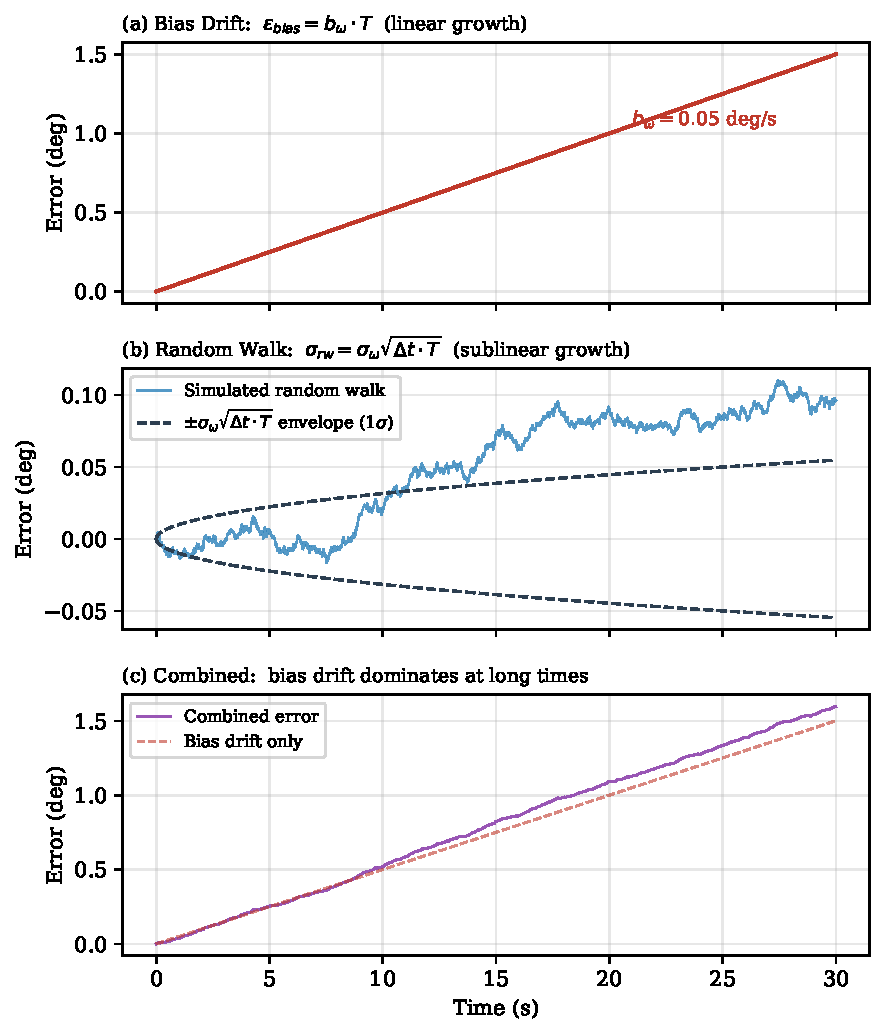
\includegraphics[width=\columnwidth]{gyro_drift_errors.pdf}
  \caption{Simulated gyroscope integration errors over 30~seconds
           ($b_\omega = 0.05$~deg/s, $\sigma_\omega = 0.1$~deg/s,
           $f_s = 100$~Hz).
           \textbf{(a)}~Bias drift grows linearly with time.
           \textbf{(b)}~Random walk is stochastic and grows as
           $\sigma_\omega\sqrt{\Delta t \cdot T}$ (dashed $1\sigma$ envelope,
           see Appendix~\ref{app:rw}).
           \textbf{(c)}~Combined error: the bias drift dominates at
           longer time scales.}
  \label{fig:gyro_drift}
\end{figure}

\begin{figure}[t]
  \centering
  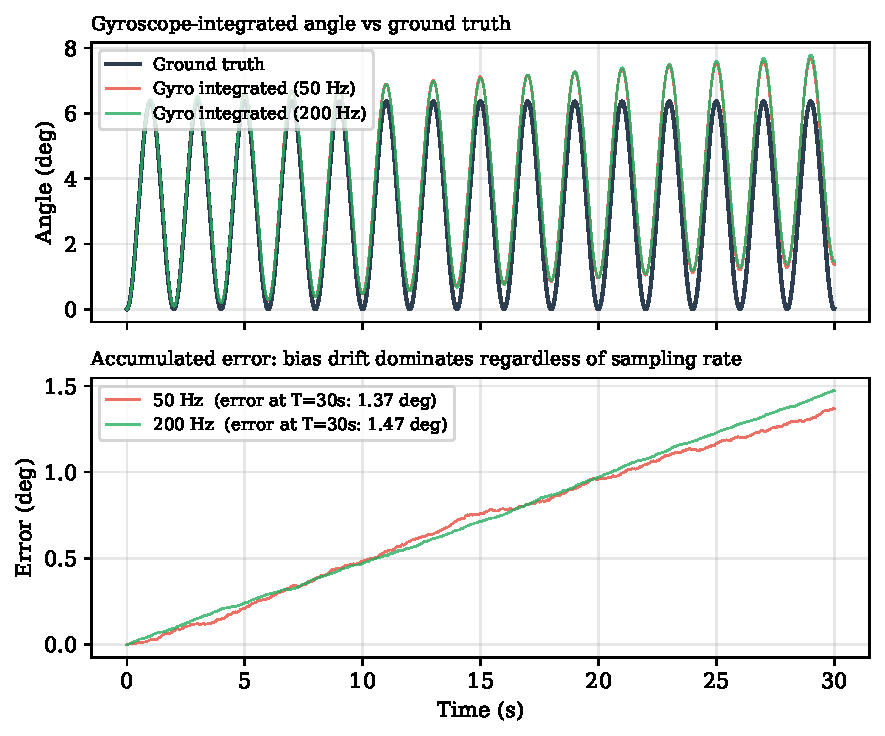
\includegraphics[width=\columnwidth]{gyro_sampling_comparison.pdf}
  \caption{Effect of sampling frequency on gyroscope integration.
           \textbf{Top:} integrated angle at 50~Hz and 200~Hz compared to
           ground truth.
           \textbf{Bottom:} accumulated error. Higher sampling rates
           reduce discretisation error but cannot eliminate bias drift,
           which depends only on $b_\omega$ and elapsed time~$T$.}
  \label{fig:gyro_sampling}
\end{figure}

\subsection{Magnetometer: Heading from Earth's Magnetic Field}
\label{sec:frames:mag}

\subsubsection{Sensor model}

A tri-axial magnetometer measures the Earth's magnetic field vector expressed
in the body frame:

\begin{equation}
  \mathbf{m}_b = R^{-1}\,\mathbf{m}_w + \mathbf{b}_m + \mathbf{n}_m
  \label{eq:mag_model}
\end{equation}

\noindent where $\mathbf{m}_w$ is the local geomagnetic field vector in the
world frame, $R$ is the rotation matrix from $\mathcal{W}$ to $\mathcal{B}$,
$\mathbf{b}_m$ is a bias term caused by hard-iron distortions (nearby
ferromagnetic materials), and $\mathbf{n}_m$ is additive noise.

In the ENU convention, the geomagnetic field has a horizontal component
pointing approximately toward magnetic North (along $Y_w$) and a vertical
component whose sign and magnitude depend on the latitude (the
\emph{inclination} angle). At mid-latitudes, the field magnitude is typically
$25$--$65~\mu$T.

\subsubsection{Why the accelerometer cannot observe yaw}
\label{sec:frames:mag:why}

As derived in Section~\ref{sec:frames:accel:derivation}, the accelerometer
measures the projection of the gravity vector onto the body axes. Gravity is
a \emph{vertical} vector: $\mathbf{g} = [0,\;0,\;g]^\top$ in the world
frame. A rotation about the vertical axis (yaw, $\psi$) leaves this vector
\emph{invariant}:

\begin{equation}
  R_z(\psi)\,\mathbf{g}
  = \begin{bmatrix}
      \cos\psi & -\sin\psi & 0 \\
      \sin\psi & \cos\psi  & 0 \\
      0        & 0         & 1
    \end{bmatrix}
  \begin{bmatrix} 0 \\ 0 \\ g \end{bmatrix}
  = \begin{bmatrix} 0 \\ 0 \\ g \end{bmatrix}
  \label{eq:yaw_gravity_invariant}
\end{equation}

\noindent Regardless of the value of $\psi$, the accelerometer reading does
not change. Therefore, \textbf{yaw is unobservable from gravity alone}.

\paragraph{Important clarification: world yaw vs.\ body-axis rotation.}
The unobservable degree of freedom is always the rotation about the
\emph{world} vertical axis (the direction of~$\mathbf{g}$), not about the
body-frame $Z_b$~axis. When the device is held horizontally---as in a
drone---$Z_b$ is aligned with gravity, so a rotation about $Z_b$ coincides
with world yaw and is entirely invisible to the accelerometer. However, when
the device is tilted (e.g.\ a smartphone held upright), $Z_b$ is no longer
parallel to~$\mathbf{g}$. In that configuration, a rotation about $Z_b$
\emph{does} change the gravity projection and is therefore partially
observable. Nevertheless, there remains exactly \textbf{one unobservable
degree of freedom}---the rotation about the gravity vector---regardless of
device orientation. It is this world-frame yaw that the magnetometer must
resolve.

This is the fundamental reason why a two-sensor (accelerometer + gyroscope)
fusion pipeline cannot fully determine orientation: the gyroscope can track
yaw changes in the short term, but its estimate drifts without any absolute
reference to correct it.

\subsubsection{Heading derivation from the magnetometer}
\label{sec:frames:mag:heading}

The Earth's magnetic field, unlike gravity, has a significant \emph{horizontal}
component that changes direction with yaw rotations. To extract the heading
angle, the magnetometer reading must first be \emph{tilt-compensated} using
the known roll and pitch angles (obtained from the accelerometer or the
complementary filter). The procedure is:

\paragraph{Step 1: Tilt compensation.}
Rotate the raw magnetometer vector from the (tilted) body frame into the
horizontal plane using the inverse of the roll and pitch rotations:

\begin{equation}
  \begin{bmatrix} m_x' \\ m_y' \\ m_z' \end{bmatrix}
  = R_x(-\phi)\;R_y(-\theta)\;
  \begin{bmatrix} m_x \\ m_y \\ m_z \end{bmatrix}
  \label{eq:tilt_compensation}
\end{equation}

\noindent Expanding the matrix product, the tilt-compensated horizontal
components are:

\begin{align}
  m_x' &= m_x\cos\theta + m_y\sin\phi\sin\theta
         + m_z\cos\phi\sin\theta
  \label{eq:mx_comp} \\[4pt]
  m_y' &= m_y\cos\phi - m_z\sin\phi
  \label{eq:my_comp}
\end{align}

\paragraph{Step 2: Compute heading.}
The yaw angle is the bearing of the horizontal magnetic component:

\begin{equation}
  \boxed{\;\psi = \arctan2\!\bigl(-m_x',\; m_y'\bigr)\;}
  \label{eq:yaw_mag}
\end{equation}

\noindent The $\arctan2$ function returns a full-circle result in
$(-180°, 180°]$, resolving the quadrant ambiguity. Note that
$\psi = 0$ corresponds to magnetic North.

\subsubsection{Limitations of the magnetometer}
\label{sec:frames:mag:limitations}

\begin{itemize}
  \item \textbf{Soft- and hard-iron distortions.} Ferromagnetic materials
        near the sensor (e.g.\ a phone case with a magnetic clasp, a metal
        table) create constant offsets (hard-iron) or directional scaling
        (soft-iron) that corrupt the reading. Calibration---typically an
        ellipsoid fit---is required before use.
  \item \textbf{Low bandwidth.} The geomagnetic field changes slowly;
        consumer magnetometers are typically sampled at 50--100~Hz but the
        useful signal content is below $\sim$\!1~Hz. High-frequency heading
        changes are better tracked by the gyroscope.
  \item \textbf{Indoor interference.} Electronic devices, power cables, and
        reinforced-concrete structures generate local magnetic anomalies that
        can cause heading errors of tens of degrees.
\end{itemize}

\noindent Despite these limitations, the magnetometer is the \emph{only}
passive sensor available on a consumer device that provides an absolute
heading reference. Its role in the fusion pipeline is strictly analogous to
that of the accelerometer for tilt: it supplies a low-frequency, drift-free
yaw reference that is fused with the high-frequency gyroscope estimate via
the complementary filter.

\subsection{The Need for Fusion}
\label{sec:frames:fusion_need}

The preceding analysis reveals a natural complementarity among the three
sensors, summarised in Table~\ref{tab:sensor_comparison}:

\begin{itemize}
  \item The \textbf{accelerometer} provides an absolute tilt reference
        (gravity) that is \emph{bounded} in error---it never drifts---but is
        only valid when the sensor is at rest or in uniform motion.
        During transients it is unreliable; once the motion ends, it
        \emph{recovers}. It \emph{cannot} observe yaw.
  \item The \textbf{magnetometer} provides an absolute heading reference
        (Earth's magnetic field) that is also bounded in error and
        self-correcting, but is sensitive to local magnetic disturbances and
        has low bandwidth.
  \item The \textbf{gyroscope} tracks rotations on \emph{all three axes}
        faithfully during fast, dynamic motion, but its integrated angle
        \emph{drifts without bound} due to bias accumulation. It never
        self-corrects.
\end{itemize}

\noindent In the frequency domain, the accelerometer and magnetometer are
reliable \emph{low-frequency} sources (slow, steady orientation on
tilt and heading respectively), while the gyroscope is a reliable
\emph{high-frequency} source (fast changes on all axes). A well-designed
fusion algorithm should retain the low-frequency content of the absolute
sensors and the high-frequency content of the gyroscope, discarding the
noisy high-frequency accelerometer/magnetometer data and the drifting
low-frequency gyroscope data. This is precisely what the complementary
filter achieves (Section~\ref{sec:complementary_filter}).

\begin{table}[t]
  \centering
  \caption{Complementary characteristics of the three sensors for
           full attitude estimation.}
  \label{tab:sensor_comparison}
  \resizebox{\columnwidth}{!}{%
  \begin{tabular}{@{}lccc@{}}
    \toprule
    \textbf{Property} & \textbf{Accel.} & \textbf{Magnet.} & \textbf{Gyro.} \\
    \midrule
    Measures            & Specific force  & Magnetic field    & Angular vel.    \\
    Provides            & Roll, Pitch     & Yaw (heading)     & Roll, Pitch, Yaw \\
    Angle via           & Trigonometry    & $\arctan2$        & Integration     \\
    Low-freq.\ acc.     & High (gravity)  & High (mag.\ field)& Low (drift)     \\
    High-freq.\ acc.    & Low (dyn.\ acc.)& Low (noise)       & High            \\
    Absolute ref.       & Yes             & Yes               & No              \\
    Affected by motion  & Yes             & No                & No              \\
    Affected by env.    & No              & Yes (mag.\ anom.) & No              \\
    Drift               & None (bounded)  & None (bounded)    & Unbounded       \\
    Self-correcting     & Yes             & Yes               & No              \\
    \bottomrule
  \end{tabular}%
  }
\end{table}

% ----- FIGURE: sensor summary -----
% TODO: Side-by-side qualitative comparison:
%   Left panel  - "Accelerometer angle": noisy around true value,
%                  spikes during motion, returns after.
%   Right panel - "Gyroscope angle": smooth, tracks true value initially,
%                  but slowly diverges (drift).
%   Annotation:  arrow pointing to "fusion zone" where both contribute.
%
% \begin{figure}[t]
%   \centering
%   \includegraphics[width=\columnwidth]{sensor_summary.pdf}
%   \caption{Qualitative comparison of angle estimates.
%            \textbf{Left:} the accelerometer is accurate at rest but
%            corrupted during motion; it always recovers.
%            \textbf{Right:} the gyroscope is smooth and responsive but
%            drifts indefinitely. Fusing both yields the best of each.}
%   \label{fig:sensor_summary}
% \end{figure}
          % 2. Reference Frames and Sensor Models
\section{Quaternion Algebra}
\label{sec:quaternions}

% ----------------------------------------------------------------
% 7 subsections: motivation, definition, rotation proof,
% geometric interpretation, rotation matrix, integration, advantages.
% ----------------------------------------------------------------

% ============================================================
%  3.1  Motivation: rotations as numbers
% ============================================================
\subsection{Motivation: Rotations as Numbers}
\label{sec:quat:motivation}

Before introducing quaternions, it is instructive to recall how
\emph{complex numbers} encode rotations in two dimensions.  A point
$(x,y)\in\mathbb{R}^2$ can be identified with the complex number
$z = x + iy$.  Multiplying $z$ by the unit complex number
$e^{i\theta} = \cos\theta + i\sin\theta$ yields

\begin{equation}
  z' \;=\; e^{i\theta}\,z
     \;=\; (x\cos\theta - y\sin\theta)
          + i\,(x\sin\theta + y\cos\theta),
  \label{eq:complex_rotation}
\end{equation}

\noindent which is exactly the rotation of $(x,y)$ by an angle $\theta$.
For example, rotating the point $(1,0)$ by $90^\circ$ amounts to multiplying
$z=1$ by $e^{i\pi/2} = i$, which gives $z'= i$, corresponding to the
point $(0,1)$---precisely the expected result.

A natural question arises: \emph{does an analogous number system exist
for rotations in $\mathbb{R}^3$?}  One might expect that three imaginary
units suffice, but William Rowan Hamilton showed in 1843 that a consistent
non-commutative algebra requires \textbf{four} components---one real and
three imaginary---giving rise to the \emph{quaternions}
$\mathbb{H} = \{q_w + q_x\mathbf{i} + q_y\mathbf{j} + q_z\mathbf{k}\}$.
Just as the unit complex numbers $e^{i\theta}$ parametrise $\mathrm{SO}(2)$,
the unit quaternions provide a double cover of $\mathrm{SO}(3)$: every
rotation in three-dimensional space can be expressed as a quaternion
conjugation, as we shall demonstrate in the following subsections.

% ============================================================
%  3.2  Definition and operations  (existing content, preserved)
% ============================================================
\subsection{Definition and Key Operations}
\label{sec:quat:def}

A quaternion $\mathbf{q}$ is a four-dimensional hypercomplex number:

\begin{equation}
  \mathbf{q} = q_w + q_x\,\mathbf{i} + q_y\,\mathbf{j} + q_z\,\mathbf{k}
             = \begin{bmatrix} q_w \\ q_x \\ q_y \\ q_z \end{bmatrix}
  \label{eq:quat_def}
\end{equation}

\noindent where $q_w$ is the \emph{scalar} (or real) part and
$(q_x, q_y, q_z)$ is the \emph{vector} (or imaginary) part. The basis
elements satisfy the fundamental relations $\mathbf{i}^2 = \mathbf{j}^2 =
\mathbf{k}^2 = \mathbf{i}\mathbf{j}\mathbf{k} = -1$.

\paragraph{Norm.}
$\|\mathbf{q}\| = \sqrt{q_w^2 + q_x^2 + q_y^2 + q_z^2}$.
A \emph{unit quaternion} satisfies $\|\mathbf{q}\| = 1$.

\paragraph{Conjugate.}
$\mathbf{q}^* = q_w - q_x\,\mathbf{i} - q_y\,\mathbf{j} - q_z\,\mathbf{k}$.
For unit quaternions, $\mathbf{q}^* = \mathbf{q}^{-1}$.

\paragraph{Hamilton product.}
Given $\mathbf{p} = (p_w, p_x, p_y, p_z)$ and
$\mathbf{q} = (q_w, q_x, q_y, q_z)$, their product $\mathbf{r} =
\mathbf{p} \otimes \mathbf{q}$ is:

\begin{equation}
  \mathbf{r} = \begin{bmatrix}
    p_w q_w - p_x q_x - p_y q_y - p_z q_z \\
    p_w q_x + p_x q_w + p_y q_z - p_z q_y \\
    p_w q_y - p_x q_z + p_y q_w + p_z q_x \\
    p_w q_z + p_x q_y - p_y q_x + p_z q_w
  \end{bmatrix}^\top
  \label{eq:hamilton}
\end{equation}

\noindent Note that the Hamilton product is \emph{not} commutative:
$\mathbf{p} \otimes \mathbf{q} \neq \mathbf{q} \otimes \mathbf{p}$ in general.

% ============================================================
%  3.3  Unit quaternion as a rotation in R^3  (rewritten)
% ============================================================
\subsection{The Unit Quaternion as a Rotation in $\mathbb{R}^3$}
\label{sec:quat:rotation}

A unit quaternion $\mathbf{q}$ encodes a rotation by angle~$\theta$ about a
unit axis~$\hat{\mathbf{u}}$:

\begin{equation}
  \mathbf{q} = \cos\frac{\theta}{2}
             + \sin\frac{\theta}{2}\,
               (u_x\,\mathbf{i} + u_y\,\mathbf{j} + u_z\,\mathbf{k})
  \label{eq:axis_angle}
\end{equation}

To rotate a vector $\mathbf{v} \in \mathbb{R}^3$, we embed it as a pure
quaternion $\mathbf{v}_q = (0, v_x, v_y, v_z)$ and compute:

\begin{equation}
  \mathbf{v}'_q = \mathbf{q} \otimes \mathbf{v}_q \otimes \mathbf{q}^*
  \label{eq:rotation}
\end{equation}

\noindent The vector part of $\mathbf{v}'_q$ is the rotated vector
$\mathbf{v}' \in \mathbb{R}^3$.  We now prove that this conjugation is
indeed a rotation---that is, an element of $\mathrm{SO}(3)$.

\paragraph{Preservation of norms.}
The norm of a quaternion product satisfies
$\|\mathbf{p}\otimes\mathbf{q}\| = \|\mathbf{p}\|\,\|\mathbf{q}\|$.
Since $\|\mathbf{q}\|=\|\mathbf{q}^*\|=1$, we obtain
\begin{equation}
  \|\mathbf{v}'_q\|
  = \|\mathbf{q}\otimes\mathbf{v}_q\otimes\mathbf{q}^*\|
  = \|\mathbf{q}\|\;\|\mathbf{v}_q\|\;\|\mathbf{q}^*\|
  = \|\mathbf{v}_q\|,
  \label{eq:norm_preservation}
\end{equation}
so the map preserves the length of every vector.

\paragraph{Linearity.}
For any scalars $\alpha,\beta\in\mathbb{R}$ and pure quaternions
$\mathbf{v}_q,\mathbf{w}_q$:
\begin{equation}
  \mathbf{q}\otimes(\alpha\mathbf{v}_q+\beta\mathbf{w}_q)\otimes\mathbf{q}^*
  = \alpha\,(\mathbf{q}\otimes\mathbf{v}_q\otimes\mathbf{q}^*)
  + \beta\,(\mathbf{q}\otimes\mathbf{w}_q\otimes\mathbf{q}^*),
  \label{eq:linearity}
\end{equation}
which follows from the bilinearity of the Hamilton product.  Hence the map
$\mathbf{v}\mapsto\mathbf{q}\otimes\mathbf{v}_q\otimes\mathbf{q}^*$
defines a linear transformation $\mathbb{R}^3\to\mathbb{R}^3$.

\paragraph{Preservation of orientation.}
A norm-preserving linear map is an \emph{orthogonal} transformation, so
its determinant is $\pm 1$.  Because the set of unit quaternions is
connected (it is the 3-sphere $S^3$) and $\mathbf{q}=1$ (the identity
quaternion) produces the identity map with $\det=+1$, and the determinant
is a continuous function of $\mathbf{q}$, we conclude that
$\det=+1$ for \emph{every} unit quaternion.  Therefore the conjugation
in~\eqref{eq:rotation} is a \textbf{proper rotation}, i.e.\ an element
of $\mathrm{SO}(3)$.

% ============================================================
%  3.4  Geometric interpretation: parallel/perpendicular decomposition
% ============================================================
\subsection{Geometric Interpretation}
\label{sec:quat:geometry}

The proof above establishes \emph{that} the conjugation is a rotation.
We now show \emph{how} it acts geometrically, which also explains the
factor $\theta/2$ in the quaternion parametrisation.

Let $\hat{\mathbf{u}}$ be the rotation axis and decompose an arbitrary
vector $\mathbf{v}$ into its parallel and perpendicular components with
respect to $\hat{\mathbf{u}}$:
\begin{equation}
  \mathbf{v} = \mathbf{v}_\parallel + \mathbf{v}_\perp,
  \qquad
  \mathbf{v}_\parallel = (\mathbf{v}\cdot\hat{\mathbf{u}})\,\hat{\mathbf{u}},
  \qquad
  \mathbf{v}_\perp = \mathbf{v} - \mathbf{v}_\parallel.
  \label{eq:decomposition}
\end{equation}

\paragraph{Parallel component is invariant.}
Because $\mathbf{v}_\parallel$ is collinear with $\hat{\mathbf{u}}$, and
$\hat{\mathbf{u}}$ commutes with every quaternion whose vector part is
proportional to $\hat{\mathbf{u}}$ (in particular with
$\mathbf{q}=\cos(\theta/2)+\sin(\theta/2)\,\hat{\mathbf{u}}$), we have:
\begin{equation}
  \mathbf{q}\otimes(\mathbf{v}_\parallel)_q\otimes\mathbf{q}^*
  = (\mathbf{v}_\parallel)_q.
  \label{eq:parallel_invariant}
\end{equation}
In other words, the component along the rotation axis is unchanged.

\paragraph{Perpendicular component is rotated by $\theta$.}
For the perpendicular component, the double-sided multiplication produces:
\begin{equation}
  \mathbf{q}\otimes(\mathbf{v}_\perp)_q\otimes\mathbf{q}^*
  = \cos\theta\;\mathbf{v}_\perp
  + \sin\theta\;(\hat{\mathbf{u}}\times\mathbf{v}_\perp),
  \label{eq:perp_rotation}
\end{equation}
which is Rodrigues' rotation formula restricted to vectors orthogonal
to the axis.  The key insight is that \emph{each} multiplication by
$\mathbf{q}$ or $\mathbf{q}^*$ contributes a half-angle rotation, so the
two multiplications together produce the full angle~$\theta$.  This is
precisely why the quaternion uses $\theta/2$ rather than $\theta$: the
\textbf{double-sided conjugation doubles the angle}.

Combining both components, we recover Rodrigues' formula for an arbitrary
vector:
\begin{equation}
  \mathbf{v}' = \cos\theta\;\mathbf{v}
              + (1-\cos\theta)\,(\mathbf{v}\cdot\hat{\mathbf{u}})\,\hat{\mathbf{u}}
              + \sin\theta\;(\hat{\mathbf{u}}\times\mathbf{v}).
  \label{eq:rodrigues}
\end{equation}

% ============================================================
%  3.5  Equivalence with the rotation matrix R(q)
% ============================================================
\subsection{Equivalence with the Rotation Matrix}
\label{sec:quat:matrix}

By expanding the conjugation
$\mathbf{q}\otimes\mathbf{v}_q\otimes\mathbf{q}^*$ component by component
using the Hamilton product~\eqref{eq:hamilton} and grouping terms in
$v_x$, $v_y$, $v_z$, one obtains the equivalent matrix form
$\mathbf{v}' = R(\mathbf{q})\,\mathbf{v}$, where:

\begin{equation}
  R(\mathbf{q}) = \begin{bmatrix}
    1 - 2(q_y^2+q_z^2)  & 2(q_x q_y - q_w q_z)  & 2(q_x q_z + q_w q_y) \\[4pt]
    2(q_x q_y + q_w q_z) & 1 - 2(q_x^2+q_z^2)    & 2(q_y q_z - q_w q_x) \\[4pt]
    2(q_x q_z - q_w q_y) & 2(q_y q_z + q_w q_x)   & 1 - 2(q_x^2+q_y^2)
  \end{bmatrix}
  \label{eq:rotation_matrix}
\end{equation}

\noindent This matrix is used whenever an explicit $3\times 3$ rotation is
needed---for instance, to project accelerometer readings into the world
frame.

\paragraph{Verification.}
One can verify that $R(\mathbf{q})$ is orthogonal and proper:
\begin{enumerate}
  \item \textbf{Orthogonality}: $R(\mathbf{q})^\top R(\mathbf{q}) = I$,
    which follows from the unit-norm constraint $q_w^2+q_x^2+q_y^2+q_z^2=1$.
  \item \textbf{Unit determinant}: $\det R(\mathbf{q}) = +1$, confirming
    that $R(\mathbf{q})\in\mathrm{SO}(3)$.
\end{enumerate}

\noindent Note that $\mathbf{q}$ and $-\mathbf{q}$ yield the same
rotation matrix $R(\mathbf{q}) = R(-\mathbf{q})$, reflecting the
\emph{double cover} of $\mathrm{SO}(3)$ by the unit quaternions.

% ============================================================
%  3.6  Integration from angular velocity  (existing content, preserved)
% ============================================================
\subsection{Quaternion Integration from Angular Velocity}
\label{sec:quat:integration}

Given the current orientation quaternion $\mathbf{q}(t)$ and a gyroscope
reading $\boldsymbol{\omega}_b = (\omega_x, \omega_y, \omega_z)$, the
orientation evolves according to the differential equation:

\begin{equation}
  \dot{\mathbf{q}}(t) = \frac{1}{2}\,\mathbf{q}(t) \otimes
  \boldsymbol{\omega}_q
  \label{eq:quat_diff}
\end{equation}

\noindent where $\boldsymbol{\omega}_q = (0, \omega_x, \omega_y, \omega_z)$ is
the angular velocity expressed as a pure quaternion. Using a first-order
discretisation with time step~$\Delta t$:

\begin{equation}
  \mathbf{q}(t + \Delta t) = \mathbf{q}(t) + \frac{\Delta t}{2}\,
  \mathbf{q}(t) \otimes \boldsymbol{\omega}_q
  \label{eq:quat_euler}
\end{equation}

\noindent After each update, $\mathbf{q}$ must be renormalised to remain on the
unit sphere: $\mathbf{q} \leftarrow \mathbf{q} / \|\mathbf{q}\|$.

% ============================================================
%  3.7  Advantages over Euler angles and matrices
% ============================================================
\subsection{Advantages over Euler Angles and Rotation Matrices}
\label{sec:quat:advantages}

Table~\ref{tab:rotation_comparison} summarises the key properties of the
three most common rotation representations.  Quaternions offer the best
trade-off between compactness, numerical stability, and computational cost
for real-time sensor fusion applications.

\begin{table}[t]
  \centering
  \caption{Comparison of rotation representations.}
  \label{tab:rotation_comparison}
  \small
  \begin{tabular}{@{}lccc@{}}
    \toprule
    \textbf{Property} & \textbf{Euler} & \textbf{Matrix} & \textbf{Quaternion} \\
    \midrule
    Parameters             & 3     & 9     & 4 \\
    Gimbal lock            & Yes   & No    & No \\
    Singularity-free       & No    & Yes   & Yes \\
    Composition cost       & High  & $O(27)$ & $O(16)$ \\
    Renormalisation        & ---   & $O(n^3)$ & $O(n)$ \\
    Interpolation (SLERP)  & Poor  & Poor  & Native \\
    \bottomrule
  \end{tabular}
\end{table}

Euler angles, while intuitive, suffer from \emph{gimbal lock}---a
singularity that occurs when two rotation axes become aligned, causing a
loss of one degree of freedom.  Rotation matrices are singularity-free
but use nine parameters (with six orthogonality constraints), making
renormalisation expensive.  Quaternions use only four parameters (with
one constraint $\|\mathbf{q}\|=1$), avoid gimbal lock entirely, compose
efficiently via the Hamilton product, and support smooth interpolation
through spherical linear interpolation (SLERP).  These properties make
quaternions the natural choice for the sensor fusion pipeline developed
in this work.
         % 3. Quaternion Algebra
\section{Complementary Filter for Attitude Estimation}
\label{sec:complementary_filter}

% ----------------------------------------------------------------
% TARGET: ~1.5 pages. The core fusion algorithm.
% ----------------------------------------------------------------

\subsection{Intuition}
\label{sec:cf:intuition}

As discussed in Section~\ref{sec:frames:fusion_need}, the accelerometer and
gyroscope have complementary noise characteristics. The key insight is that
their useful information occupies \emph{different frequency bands}:

\begin{itemize}
  \item The accelerometer-derived angle is reliable at \textbf{low frequencies}
        (below $\sim$\!1~Hz) but corrupted at high frequencies.
  \item The gyroscope-integrated angle is reliable at \textbf{high frequencies}
        but drifts at low frequencies.
\end{itemize}

A complementary filter combines the two by applying a \emph{low-pass filter}
to the accelerometer and a \emph{high-pass filter} to the gyroscope, such
that their transfer functions sum to unity across all frequencies.

\subsection{Filter Derivation}
\label{sec:cf:derivation}

Let $\theta_a(t)$ denote the tilt angle estimated from the accelerometer and
$\theta_g(t)$ the angle obtained by integrating the gyroscope. The
complementary filter output is:

\begin{equation}
  \boxed{
    \hat{\theta}(t) = \alpha \bigl[\hat{\theta}(t - \Delta t)
    + \omega(t)\,\Delta t\bigr]
    + (1 - \alpha)\,\theta_a(t)
  }
  \label{eq:comp_filter}
\end{equation}

\noindent where $\alpha \in (0, 1)$ is the filter coefficient. The first term
is a \emph{high-pass filter} on the gyroscope (it propagates the previous
estimate forward and adds the incremental rotation), and the second term is a
\emph{low-pass filter} on the accelerometer (it slowly corrects toward the
gravity reference).

The time constant of the filter is:

\begin{equation}
  \tau = \frac{\alpha\,\Delta t}{1 - \alpha}
  \label{eq:time_constant}
\end{equation}

\noindent Typical values are $\alpha = 0.96$--$0.98$, corresponding to time
constants of a few seconds.

% ----- FIGURE: complementary filter block diagram -----
% TODO: Block diagram showing:
%   - Gyroscope → integrator → HPF ──┐
%   - Accelerometer → atan2 → LPF ──┤→ Σ → θ_hat
%   - Labels: α and (1-α)
%   - Frequency response subplot below
%
% \begin{figure}[t]
%   \centering
%   \includegraphics[width=\columnwidth]{complementary_filter.pdf}
%   \caption{Block diagram of the complementary filter. The gyroscope path
%            (top) acts as a high-pass filter with coefficient $\alpha$; the
%            accelerometer path (bottom) acts as a low-pass filter with
%            coefficient $(1-\alpha)$. Their sum reconstructs the full-band
%            attitude estimate.}
%   \label{fig:comp_filter}
% \end{figure}

\subsection{Accelerometer Tilt Extraction}
\label{sec:cf:tilt}

When the sensor is approximately stationary, the accelerometer measures the
gravity vector projected onto the body axes. The roll and pitch angles can be
extracted as:

\begin{align}
  \phi   &= \arctan\!\left(\frac{a_y}{\sqrt{a_x^2 + a_z^2}}\right)
  \label{eq:roll} \\[4pt]
  \theta &= \arctan\!\left(\frac{-a_x}{\sqrt{a_y^2 + a_z^2}}\right)
  \label{eq:pitch}
\end{align}

\noindent These relations assume that the only force acting on the sensor is
gravity. During dynamic motion, the estimates become unreliable---precisely the
regime where the gyroscope takes over through the high-pass path.

\subsection{Quaternion Form of the Complementary Filter}
\label{sec:cf:quaternion}

To avoid gimbal lock, the complementary filter is implemented in quaternion
space. At each time step:

\begin{enumerate}
  \item Integrate the gyroscope to obtain a predicted quaternion
        $\mathbf{q}_\text{pred}$ using Eq.~\eqref{eq:quat_euler}.
  \item Compute a reference quaternion $\mathbf{q}_\text{acc}$ from the
        accelerometer tilt angles (Eqs.~\ref{eq:roll}--\ref{eq:pitch}).
  \item Blend the two using spherical linear interpolation (SLERP):
\end{enumerate}

\begin{equation}
  \mathbf{q}(t) = \text{SLERP}\bigl(\mathbf{q}_\text{acc},\;
                  \mathbf{q}_\text{pred},\; \alpha\bigr)
  \label{eq:slerp_filter}
\end{equation}

\noindent This is the quaternion analogue of the scalar
Eq.~\eqref{eq:comp_filter}, with the SLERP parameter playing the role of
$\alpha$.
      % 4. Complementary Filter
\section{Gradient-Descent Attitude Estimation: The Madgwick Filter}
\label{sec:madgwick}

% ----------------------------------------------------------------
% Motivation, derivation, and comparison with the complementary filter.
% ----------------------------------------------------------------

The complementary filter presented in Section~\ref{sec:complementary_filter}
provides an effective and intuitive approach to sensor fusion.  However, its
scalar formulation operates on Euler angles independently, which introduces
two practical limitations: (i)~the relationship between body-frame angular
velocities and Euler angle rates is \emph{nonlinear and coupled} (requiring
explicit Euler rate equations), and (ii)~the representation becomes singular
near $\pm 90^\circ$ pitch (gimbal lock).  While the quaternion form of the
complementary filter (Section~\ref{sec:cf:quaternion}) addresses these issues
in principle via SLERP blending, an alternative family of algorithms performs
the fusion \emph{natively} in quaternion space using gradient descent on an
orientation error objective.  The most widely adopted of these is the filter
proposed by Madgwick et al.~(2011), which we describe in this section.

\subsection{Problem Statement}
\label{sec:madg:problem}

Given a stream of gyroscope readings
$\boldsymbol{\omega}_b \in \mathbb{R}^3$, accelerometer readings
$\mathbf{a}_b \in \mathbb{R}^3$, and (optionally) magnetometer readings
$\mathbf{m}_b \in \mathbb{R}^3$, we seek the unit quaternion
$\mathbf{q}(t)$ that represents the orientation of the sensor body frame
with respect to a fixed world frame at each time step.

The key idea is to formulate attitude estimation as an \emph{optimisation
problem}: find the quaternion that best aligns the sensor measurements with
known reference directions in the world frame (gravity and the geomagnetic
field).

\subsection{Gyroscope Prediction}
\label{sec:madg:gyro}

As in the complementary filter, the gyroscope provides a short-term
orientation prediction.  Given the current estimate $\mathbf{q}(t)$ and the
angular velocity $\boldsymbol{\omega}_b(t)$, the predicted quaternion is
obtained by integrating the quaternion kinematic equation
(Eq.~\ref{eq:quat_euler}):

\begin{equation}
  \mathbf{q}_{\omega}(t + \Delta t)
  = \mathbf{q}(t)
    + \frac{\Delta t}{2}\,\mathbf{q}(t) \otimes \boldsymbol{\omega}_q(t)
  \label{eq:madg_gyro}
\end{equation}

\noindent where $\boldsymbol{\omega}_q = (0,\, \omega_x,\, \omega_y,\,
\omega_z)$.  This step is identical to the gyroscope path in the
complementary filter and inherits the same drift characteristics.

\subsection{Accelerometer and Magnetometer Correction via Gradient Descent}
\label{sec:madg:gradient}

The correction step is where the Madgwick filter fundamentally differs from
the complementary filter.  Instead of extracting Euler angles from the
accelerometer and blending them with the gyroscope output, the Madgwick
filter defines an \emph{objective function} whose minimum corresponds to the
correct orientation.

\subsubsection{Objective Function (IMU: Accelerometer Only)}

Let $\hat{\mathbf{d}}_w = (0,\, 0,\, 1)^\top$ be the expected direction of
gravity in the world frame (normalised).  If the true orientation is
$\mathbf{q}$, then the accelerometer should measure:

\begin{equation}
  \hat{\mathbf{a}}_b = \mathbf{q}^* \otimes \hat{\mathbf{d}}_{w,q}
                       \otimes \mathbf{q}
  \label{eq:expected_accel}
\end{equation}

\noindent The error between the predicted and actual normalised accelerometer
reading $\hat{\mathbf{a}}_b^{\,\text{meas}}$ defines the objective function:

\begin{equation}
  f(\mathbf{q})
  = \mathbf{q}^* \otimes \hat{\mathbf{d}}_{w,q} \otimes \mathbf{q}
    - \hat{\mathbf{a}}_{b,q}^{\,\text{meas}}
  \label{eq:objective}
\end{equation}

\noindent where $f : \mathbb{R}^4 \to \mathbb{R}^3$ maps a quaternion to the
residual between the expected and observed gravity direction.  The optimal
orientation satisfies $f(\mathbf{q}) = \mathbf{0}$.

\subsubsection{Gradient Step}

Rather than solving the full nonlinear optimisation, Madgwick applies a
\emph{single gradient descent step} per time sample, which is sufficient
because the orientation changes slowly relative to the sampling rate:

\begin{equation}
  \mathbf{q}_{\nabla}(t)
  = \mathbf{q}(t)
    - \beta\,\frac{\nabla f(\mathbf{q})}{\|\nabla f(\mathbf{q})\|}
  \label{eq:gradient_step}
\end{equation}

\noindent where $\nabla f = J^\top\!(\mathbf{q})\, f(\mathbf{q})$ is
computed analytically from the Jacobian $J(\mathbf{q})$ of the objective
function with respect to the quaternion components.  The normalisation
$\|\nabla f\|$ ensures that the step magnitude depends only on $\beta$, not
on the error amplitude.

\subsubsection{Extension to MARG (with Magnetometer)}

When magnetometer data is available, the objective function is extended to
include the geomagnetic field direction.  Let $\hat{\mathbf{b}}_w$ be the
expected magnetic field direction in the world frame (computed from the
magnetometer measurement itself, projected to have zero East component).
The combined objective becomes:

\begin{equation}
  f_{\text{MARG}}(\mathbf{q})
  = \begin{bmatrix}
      f_g(\mathbf{q}) \\[2pt]
      f_b(\mathbf{q})
    \end{bmatrix}
  \label{eq:objective_marg}
\end{equation}

\noindent where $f_g$ is the gravity residual and $f_b$ is the magnetic field
residual.  The Jacobian becomes a $6 \times 4$ matrix, and the gradient step
proceeds analogously.  The magnetometer provides an absolute heading
reference that the accelerometer alone cannot observe (since gravity is
invariant under rotations about the vertical axis, as discussed in
Section~\ref{sec:proj:gravity}).

\subsection{Filter Fusion}
\label{sec:madg:fusion}

The final quaternion estimate is a weighted combination of the gyroscope
prediction and the gradient correction:

\begin{equation}
  \boxed{
    \mathbf{q}(t + \Delta t)
    = \gamma\,\mathbf{q}_{\omega}(t + \Delta t)
      + (1 - \gamma)\,\mathbf{q}_{\nabla}(t + \Delta t)
  }
  \label{eq:madg_fusion}
\end{equation}

\noindent followed by renormalisation $\mathbf{q} \leftarrow \mathbf{q} /
\|\mathbf{q}\|$.  In the original formulation, the gain parameter $\beta$
simultaneously controls the step size and the effective blending ratio,
playing a role analogous to $\alpha$ in the complementary filter.  A typical
value is $\beta = 0.041$ for MARG configurations.

The crucial difference is that \textbf{the entire fusion operates in
quaternion space}: there is no intermediate conversion to Euler angles, no
need for Euler rate equations, and no singularity at $\pm 90^\circ$ pitch.

\subsection{Comparison with the Complementary Filter}
\label{sec:madg:comparison}

Table~\ref{tab:cf_vs_madg} summarises the key differences between the two
approaches.

\begin{table}[t]
  \centering
  \caption{Complementary filter vs.\ Madgwick filter.}
  \label{tab:cf_vs_madg}
  \small
  \begin{tabular}{@{}lcc@{}}
    \toprule
    \textbf{Property}
      & \textbf{Complementary}
      & \textbf{Madgwick} \\
    \midrule
    Fusion domain
      & Euler angles
      & Quaternion \\
    Gimbal lock
      & Yes (scalar form)
      & No \\
    Euler rate equations
      & Required
      & Not needed \\
    Magnetometer fusion
      & Separate filter
      & Integrated \\
    Tuning parameters
      & $\alpha$ per axis
      & Single $\beta$ \\
    Computational cost
      & Very low
      & Low \\
    Gravity sign convention
      & Must be handled
      & Automatic \\
    \bottomrule
  \end{tabular}
\end{table}

\subsubsection{Euler Rate Coupling}

In the scalar complementary filter, the gyroscope rates
$(\omega_x, \omega_y, \omega_z)$ are used directly as the rates of change
of roll, pitch, and yaw.  This is only valid for small angles.  The correct
relationships are:

\begin{align}
  \dot{\phi}   &= \omega_x
    + \sin\phi\,\tan\theta\;\omega_y
    + \cos\phi\,\tan\theta\;\omega_z
  \label{eq:euler_rate_roll} \\[3pt]
  \dot{\theta} &= \cos\phi\;\omega_y - \sin\phi\;\omega_z
  \label{eq:euler_rate_pitch} \\[3pt]
  \dot{\psi}   &= \frac{\sin\phi}{\cos\theta}\;\omega_y
    + \frac{\cos\phi}{\cos\theta}\;\omega_z
  \label{eq:euler_rate_yaw}
\end{align}

\noindent At large inclinations (e.g.\ $\theta > 20^\circ$), ignoring this
coupling introduces significant cross-axis errors that corrupt the
orientation estimate and, consequently, the gravity removal step.  The
Madgwick filter avoids this entirely because quaternion integration
(Eq.~\ref{eq:madg_gyro}) naturally handles the nonlinear coupling
between axes without any explicit trigonometric corrections.

\subsubsection{Gravity Sign Convention}

A subtle but practically important difference concerns the sign of the
gravity vector.  The complementary filter extracts tilt angles from the
accelerometer and subtracts gravity as a scalar magnitude
$\mathbf{g}_w = (0, 0, \pm g)$, where the sign depends on the sensor
convention.  If the sensor reports $a_z \approx +9.8$~m/s$^2$ at rest
(screen up), the gravity vector must be subtracted as $(0, 0, +g)$; if it
reports $a_z \approx -9.8$~m/s$^2$ (screen down or alternate convention),
the sign must be flipped.

The Madgwick filter is immune to this issue: it works with the
\emph{normalised} accelerometer reading and optimises for the direction
of gravity, not its sign.  The gravity vector in the world frame is then
determined empirically from the calibration phase as:

\begin{equation}
  \mathbf{g}_w = \frac{1}{N_c} \sum_{n=1}^{N_c}
    \mathbf{a}_w[n]
  \label{eq:g_world_measured}
\end{equation}

\noindent where $\mathbf{a}_w[n] = \mathbf{q}[n] \otimes
\mathbf{a}_{b,q}[n] \otimes \mathbf{q}^*[n]$ is the accelerometer reading
rotated to the world frame using the Madgwick quaternion.  This approach is
robust to any sensor sign convention and eliminates a common source of
implementation errors.

\subsubsection{Effect on Position Estimation}

Because the Madgwick filter produces a more accurate orientation estimate
(especially at large inclinations), the gravity removal step is more
precise, which directly reduces the gravity leakage that dominates the
position drift.  In our experiments with a 39-second recording of repetitive
vertical hand movements (``subidas\_bajadas\_con\_pausa''), the Madgwick
pipeline produced:

\begin{itemize}
  \item A Z-axis range of $[0.00,\; 0.76]$~m, consistent with the actual
        hand movement amplitude.
  \item No negative Z values, confirming that the hand never descended below
        its starting position (as expected from the experimental protocol).
  \item Near-zero residual bias after gravity subtraction
        ($\sim 10^{-6}$~m/s$^2$), compared to biases of order $\pm 19$~m/s$^2$
        with the scalar complementary filter before sign correction.
\end{itemize}

\noindent Furthermore, the Madgwick pipeline does not require a high-pass
filter on the linear acceleration, which was previously necessary to
compensate for gravity leakage in the complementary filter approach.  The
removal of this filter is significant because the high-pass filter, while
effective at removing drift, also \emph{destroys sustained displacements}:
it forces the acceleration to have zero mean, which means any net position
change (e.g.\ moving up and staying up) is gradually pulled back toward the
origin.  This manifested as backward loops at rest positions and spurious
negative heights---artefacts that disappear entirely with the improved
orientation from the Madgwick filter.
            % 5. Madgwick Filter
\section{World-Frame Projection and Position Integration}
\label{sec:projection}

% ----------------------------------------------------------------
% TARGET: ~1 page. From quaternion to position.
% ----------------------------------------------------------------

\subsection{Rotating Acceleration to the World Frame}
\label{sec:proj:rotation}

Once the attitude quaternion $\mathbf{q}(t)$ has been estimated by the
complementary filter, each raw accelerometer reading
$\mathbf{a}_b(t)$ can be transformed into the world frame:

\begin{equation}
  \mathbf{a}_w(t) = \mathbf{q}(t) \otimes \mathbf{a}_{b,q}(t)
                    \otimes \mathbf{q}^*(t)
  \label{eq:a_world}
\end{equation}

\noindent where $\mathbf{a}_{b,q} = (0, a_x, a_y, a_z)$ is the accelerometer
reading embedded as a pure quaternion. The vector part of the result gives
$\mathbf{a}_w = (a_{w,x},\; a_{w,y},\; a_{w,z})$ in the world frame.

% ----- FIGURE: rotation illustration -----
% TODO: Illustration showing:
%   - A tilted sensor with a_body vector
%   - The quaternion rotation arrow
%   - The resulting a_world vector in the world frame
%   - Gravity subtraction step
%
% \begin{figure}[t]
%   \centering
%   \includegraphics[width=\columnwidth]{frame_rotation.pdf}
%   \caption{Projection of the body-frame acceleration into the world frame
%            via quaternion conjugation, followed by gravity removal.}
%   \label{fig:frame_rotation}
% \end{figure}

\subsection{Gravity Removal}
\label{sec:proj:gravity}

In the world frame, gravity appears as a constant vector
$\mathbf{g}_w = (0,\; 0,\; g)^\top$ (assuming ENU convention with
$g \approx 9.81\;\text{m/s}^2$). The linear acceleration is:

\begin{equation}
  \mathbf{a}_\text{lin}(t) = \mathbf{a}_w(t) - \mathbf{g}_w
  \label{eq:gravity_removal}
\end{equation}

\noindent This step is possible \emph{only} because the rotation to the world
frame has been performed first. In the body frame, the gravity component
changes direction with every rotation, making subtraction impossible.

\subsection{Double Integration to Position}
\label{sec:proj:integration}

Velocity and position are obtained by numerical integration of the
gravity-free acceleration:

\begin{align}
  \mathbf{v}(t + \Delta t) &= \mathbf{v}(t)
    + \mathbf{a}_\text{lin}(t)\,\Delta t
  \label{eq:velocity} \\[4pt]
  \mathbf{p}(t + \Delta t) &= \mathbf{p}(t)
    + \mathbf{v}(t)\,\Delta t
    + \tfrac{1}{2}\,\mathbf{a}_\text{lin}(t)\,\Delta t^2
  \label{eq:position}
\end{align}

\noindent with initial conditions $\mathbf{v}(0) = \mathbf{0}$ and
$\mathbf{p}(0) = \mathbf{0}$ (the sensor starts at rest at the origin).

\subsection{Drift in Position Estimation}
\label{sec:proj:drift}

Double integration amplifies any residual error in
$\mathbf{a}_\text{lin}$: a constant bias $\epsilon$ in acceleration produces
a position error that grows as $\frac{1}{2}\epsilon\,t^2$. This error has two
distinct sources:

\paragraph{Static bias.}
The accelerometer has a small, approximately constant offset that persists
even at rest. This can be estimated and removed during an initial calibration
phase by averaging the linear acceleration over a stationary period of
several seconds.

\paragraph{Gravity leakage from orientation error.}
This is the dominant source of drift. Even a small error $\delta$ in the
estimated roll or pitch causes the gravity vector to be imperfectly
subtracted after the world-frame rotation, leaving a residual:

\begin{equation}
  \epsilon_g \approx g \sin(\delta)
  \label{eq:gravity_leakage}
\end{equation}

\noindent For example, an orientation error of just $\delta = 1.4°$ produces
a residual of $9.81 \times \sin(1.4°) \approx 0.24$~m/s$^2$. After double
integration over a time interval $T$:

\begin{equation}
  \Delta p = \tfrac{1}{2}\,\epsilon_g\,T^2
           = \tfrac{1}{2}\,g\sin(\delta)\,T^2
  \label{eq:drift_position}
\end{equation}

\noindent For $T = 3$~s, this yields $\Delta p \approx 1.08$~m of spurious
displacement. Crucially, this error \emph{changes direction} as the device
rotates---it is not a fixed offset that can be calibrated away. It affects all
three world-frame axes (X, Y, Z), not just the vertical. This is the
fundamental limitation of inertial navigation with consumer-grade MEMS
sensors.

\subsection{Drift Mitigation Strategies}
\label{sec:proj:mitigation}

Three complementary strategies are applied to reduce the drift:

\subsubsection{Static Calibration with Measured Gravity}
\label{sec:proj:calibration}

Rather than using the textbook value $g = 9.81$~m/s$^2$, the actual gravity
magnitude is estimated from the sensor data during the initial rest phase:

\begin{equation}
  g_\text{meas} = \frac{1}{N_c} \sum_{n=1}^{N_c}
    \lVert \mathbf{a}_b[n] \rVert
  \label{eq:g_measured}
\end{equation}

\noindent where $N_c$ is the number of samples in the rest phase.
The residual linear acceleration bias is then estimated as the mean of
$\mathbf{a}_\text{lin}$ over the same interval and subtracted from the entire
signal. Using the full rest phase ($N_c \approx 1000$ samples at 100~Hz,
corresponding to $\sim$10~s) instead of a handful of samples dramatically
improves the bias estimate.

\subsubsection{Zero-Velocity Updates (ZUPT)}
\label{sec:proj:zupt}

When the sensor is stationary, its true velocity is zero. Any non-zero
integrated velocity at that instant is, by definition, accumulated error.
A \emph{zero-velocity update} exploits this constraint by resetting the
velocity to zero whenever the sensor is detected to be at rest.

\paragraph{Stationary detection.}
Two conditions must hold simultaneously over a sliding window of $W$
consecutive samples:

\begin{align}
  \bigl|\,\lVert \mathbf{a}_b[n] \rVert - g\,\bigr|
    &< \sigma_a
  \label{eq:zupt_accel} \\[4pt]
  \lVert \boldsymbol{\omega}_b[n] \rVert
    &< \sigma_\omega
  \label{eq:zupt_gyro}
\end{align}

\noindent The first condition checks that the accelerometer norm is close to
gravity (no linear acceleration). The second checks that the angular velocity
is near zero (no rotation). Requiring both conditions over a window of $W$
samples (typically $W = 5$) prevents false positives from momentary pauses in
a single channel. Typical thresholds are $\sigma_a = 0.3$~m/s$^2$ and
$\sigma_\omega = 0.15$~rad/s.

\paragraph{Velocity reset.}
At every sample classified as stationary, the integrated velocity is forced to
zero on all three axes:

\begin{equation}
  \text{if stationary}[n]: \quad \mathbf{v}[n] = \mathbf{0}
  \label{eq:zupt_reset}
\end{equation}

\noindent This prevents unbounded velocity drift during rest periods and
provides anchor points for the subsequent backward correction.

\subsubsection{Backward Velocity Correction}
\label{sec:proj:backward}

ZUPT alone resets velocity at rest, but during movement segments the velocity
still drifts due to gravity leakage. The \emph{backward correction} addresses
this by distributing the accumulated velocity error linearly across each
movement segment.

\paragraph{Segment identification.}
A movement segment is defined as the interval between two consecutive
stationary phases. Let $n_s$ be the first moving sample (where the sensor
leaves rest) and $n_e$ be the last moving sample (just before the next rest
phase begins). At $n_e$, the velocity $\mathbf{v}[n_e]$ should ideally
transition smoothly to zero, but in practice it carries an error
$\mathbf{e}_v = \mathbf{v}[n_e]$ due to drift accumulated during the segment.

\paragraph{Linear error distribution.}
The error is assumed to grow approximately linearly during the segment (since
gravity leakage acts as a roughly constant bias over short intervals). It is
therefore distributed proportionally:

\begin{equation}
  \mathbf{v}_\text{corr}[n] = \mathbf{v}[n]
    - \mathbf{e}_v \cdot \frac{n - n_s + 1}{n_e - n_s + 1},
    \quad n \in [n_s,\, n_e]
  \label{eq:backward_correction}
\end{equation}

\noindent At $n = n_s$ the correction is minimal; at $n = n_e$ the full error
is subtracted, ensuring a smooth transition to zero velocity at the next ZUPT.
The corrected velocity is then integrated to obtain the position estimate.

\paragraph{Limitations.}
The backward correction is effective when the user's motion naturally includes
pauses (e.g.\ drawing shapes with intermittent stops). However, during
continuous uninterrupted motion, no ZUPT events occur and the correction
cannot be applied. This motivates the high-pass filtering strategy described
next.

\subsubsection{High-Pass Filtering of Linear Acceleration}
\label{sec:proj:highpass}

Even after gravity subtraction and static bias removal, the linear
acceleration retains a slowly varying residual caused by orientation
estimation errors. As shown in
Section~\ref{sec:proj:drift}, an orientation error of $\delta$ produces a
gravity leakage $\epsilon_g \approx g\sin(\delta)$ that changes direction as
the device rotates but maintains a \emph{non-zero mean} over time. This
non-zero mean, when integrated twice, produces the characteristic
monotonic drift observed in position estimates.

The key insight is that \textbf{real translational acceleration has zero
mean}: every acceleration phase (push) is followed by a deceleration phase
(stop), so the integral over a complete movement cycle is approximately zero.
In contrast, gravity leakage is a low-frequency bias with non-zero mean. A
high-pass filter can therefore separate the two.

\paragraph{First-order IIR high-pass filter.}
We apply a causal first-order high-pass filter independently to each axis of
$\mathbf{a}_\text{lin}$:

\begin{equation}
  y[n] = \alpha_\text{hp}\,\bigl(y[n-1] + x[n] - x[n-1]\bigr)
  \label{eq:highpass}
\end{equation}

\noindent where $x[n]$ is the input (linear acceleration after bias removal)
and $y[n]$ is the filtered output. The parameter
$\alpha_\text{hp} \in (0,\,1)$ controls the cutoff frequency:

\begin{equation}
  f_c = \frac{1 - \alpha_\text{hp}}{2\pi\,\Delta t}
  \label{eq:hp_cutoff}
\end{equation}

\noindent Signals below $f_c$ are attenuated (including the gravity leakage
bias); signals above $f_c$ pass through (the actual motion).

\paragraph{Choosing the cutoff frequency.}
The cutoff must satisfy two constraints simultaneously:

\begin{enumerate}
  \item $f_c$ must be \textbf{above} the frequency of the gravity leakage
        bias, which is quasi-static ($\ll 1$~Hz).
  \item $f_c$ must be \textbf{below} the fundamental frequency of the actual
        motion, so that the real acceleration signal is preserved.
\end{enumerate}

\noindent The optimal value therefore depends on the \emph{type of motion},
not on the individual recording:

\begin{itemize}
  \item \textbf{Fast hand gestures} ($\sim$2--4~Hz): $\alpha_\text{hp}
        \approx 0.85$, giving $f_c \approx 2.4$~Hz at 100~Hz sampling.
  \item \textbf{Walking or slow movements} ($\sim$1--2~Hz):
        $\alpha_\text{hp} \approx 0.95$, giving $f_c \approx 0.8$~Hz.
  \item \textbf{Very slow gestures} ($< 1$~Hz): $\alpha_\text{hp}
        \approx 0.98$, giving $f_c \approx 0.3$~Hz. At this point the filter
        provides minimal benefit, as the leakage frequency overlaps with the
        motion frequency.
\end{itemize}

\noindent If $f_c$ is set too high, the filter removes part of the real
acceleration signal, causing the estimated displacement to be
\emph{underestimated}. If $f_c$ is set too low, the gravity leakage passes
through and drift reappears. In practice, $\alpha_\text{hp}$ does not need to
be re-tuned for each recording---it only needs to match the general category
of motion (fast vs.\ slow).

\paragraph{Effect on drift.}
In our experiments, adding the high-pass filter reduced the position drift
from several meters to the order of $\pm 0.2$~m for a 17-second recording of
repetitive up-and-down hand motion, even without any ZUPT corrections (no
pauses in the motion). The mean residual acceleration on the Z-axis dropped
from $+0.41$~m/s$^2$ (without filter) to $+0.02$~m/s$^2$ (with
$\alpha_\text{hp} = 0.85$).

\subsubsection{Summary of the Drift Mitigation Pipeline}
\label{sec:proj:pipeline_summary}

The complete pipeline applies five corrections in sequence:

\begin{enumerate}
  \item \textbf{Measured gravity magnitude}: $g_\text{meas}$ from the rest
        phase replaces the nominal $9.81$~m/s$^2$.
  \item \textbf{Static bias removal}: mean of
        $\mathbf{a}_\text{lin}$ during rest is subtracted.
  \item \textbf{Moving average}: a short window ($\sim$5 samples) smooths
        high-frequency noise and vibration spikes.
  \item \textbf{High-pass filter}: removes the low-frequency gravity leakage
        bias that causes monotonic drift.
  \item \textbf{Acceleration clamp}: limits $|\mathbf{a}_\text{lin}|$ to a
        physically reasonable maximum (e.g.\ $\pm 4$~m/s$^2$ for hand motion),
        rejecting residual spikes from large orientation errors.
\end{enumerate}

\noindent After filtering, ZUPT and backward velocity correction are applied
during integration when stationary phases are available. For continuous motion
without pauses, the high-pass filter alone provides the primary drift
mitigation.

% ----- FIGURE: full pipeline -----
% TODO: End-to-end block diagram:
%   [Accel] ──→ [Tilt] ──→ [LPF] ──┐
%   [Gyro]  ──→ [∫ω]  ──→ [HPF] ──┤→ [q(t)] → [Rotate a_b] → [-g] → [∫∫] → [p(t)]
%
% \begin{figure*}[t]
%   \centering
%   \includegraphics[width=\textwidth]{full_pipeline.pdf}
%   \caption{Complete signal-processing pipeline: from raw sensor data to
%            three-dimensional position. The complementary filter estimates
%            orientation; the quaternion rotation projects acceleration into
%            the world frame; double integration yields position.}
%   \label{fig:pipeline}
% \end{figure*}
             % 6. World-Frame Projection & Position
\section{Experimental Results}
\label{sec:results}

% ----------------------------------------------------------------
% TARGET: ~1 page. To be filled with real data.
% ----------------------------------------------------------------

% TODO: Fill in with actual experimental results.
% Suggested content:
%
% \subsection{Experimental Setup}
% - Device used (iPhone model, iOS version)
% - Sampling rate (e.g., 100 Hz)
% - Test scenarios (static, rotation-only, translation, combined)
% - Ground-truth method (if available)
%
% \subsection{Attitude Estimation Accuracy}
% - Compare complementary filter output vs. CoreMotion's built-in quaternion
% - Show roll/pitch/yaw over time
% - [Fig]: time-series plot of estimated vs. reference angles
%
% \subsection{Position Tracking}
% - Show 3D trajectory for a known path
% - Discuss drift over time
% - [Fig]: 3D trajectory plot
% - [Fig]: position error vs. time
%
% \subsection{Effect of Filter Coefficient}
% - Sweep alpha from 0.90 to 0.99
% - Show noise vs. drift trade-off
% - [Fig]: comparison of different alpha values

\section{Conclusions and Future Work}
\label{sec:conclusions}

% TODO: Summarise findings and outline next steps.
% Suggested content:
%
% \subsection{Summary}
% - Recap the pipeline: complementary filter → quaternion → rotation → integration
% - Highlight key advantage: singularity-free orientation with minimal computation
%
% \subsection{Future Work}
% - Extended Kalman Filter or Madgwick filter for better accuracy
% - Magnetometer integration for absolute heading
% - Map-aided or vision-aided drift correction
% - Real-time implementation analysis on iOS (latency, power consumption)
         % 7. Results & 8. Conclusions

% --- Appendices ---
\appendix

\section{Derivation of Gyroscope Integration Error Bounds}
\label{app:error_bounds}

This appendix provides a rigorous derivation of the three error terms that
arise when numerically integrating a gyroscope signal: bias drift, angular
random walk, and discretisation error. These results underpin the theoretical
envelopes shown in Figs.~\ref{fig:gyro_drift} and~\ref{fig:gyro_sampling}.

% ===================================================================
\subsection{Setup and Notation}
\label{app:setup}

Consider a single-axis gyroscope sampled at frequency $f_s = 1/\Delta t$.
At each time step $n$, the measured angular velocity is:

\begin{equation}
  \omega[n] = \omega_\text{true}[n] + b_\omega + n_\omega[n]
  \label{eq:app:gyro_model}
\end{equation}

\noindent where:
\begin{itemize}
  \item $\omega_\text{true}[n]$ is the true angular velocity,
  \item $b_\omega$ is a constant bias (deg/s),
  \item $n_\omega[n]$ are independent and identically distributed (i.i.d.)
        random variables with $E[n_\omega[n]] = 0$ and
        $\text{Var}[n_\omega[n]] = \sigma_\omega^2$.
\end{itemize}

The angle is estimated by rectangular (Euler) integration:

\begin{equation}
  \hat{\theta}[N] = \sum_{n=1}^{N} \omega[n]\,\Delta t
  \label{eq:app:integration}
\end{equation}

\noindent while the true angle is:

\begin{equation}
  \theta_\text{true}[N] = \sum_{n=1}^{N} \omega_\text{true}[n]\,\Delta t
  \label{eq:app:true_angle}
\end{equation}

The total error is the difference:

\begin{equation}
  \epsilon[N] = \hat{\theta}[N] - \theta_\text{true}[N]
              = \sum_{n=1}^{N} \bigl(b_\omega + n_\omega[n]\bigr)\,\Delta t
  \label{eq:app:total_error}
\end{equation}

\noindent We can separate this into two independent terms:

\begin{equation}
  \epsilon[N]
  = \underbrace{\sum_{n=1}^{N} b_\omega\,\Delta t}_{\epsilon_\text{bias}[N]}
  + \underbrace{\sum_{n=1}^{N} n_\omega[n]\,\Delta t}_{\epsilon_\text{rw}[N]}
  \label{eq:app:error_split}
\end{equation}

% ===================================================================
\subsection{Bias Drift: $\epsilon_\text{bias}$}
\label{app:bias}

Since $b_\omega$ is constant, the sum is trivial:

\begin{equation}
  \epsilon_\text{bias}[N]
  = \sum_{n=1}^{N} b_\omega\,\Delta t
  = N \cdot b_\omega \cdot \Delta t
  \label{eq:app:bias_sum}
\end{equation}

\noindent Substituting $T = N\,\Delta t$ (total elapsed time):

\begin{equation}
  \boxed{\;\epsilon_\text{bias} = b_\omega \cdot T\;}
  \label{eq:app:bias_final}
\end{equation}

\paragraph{Properties.}
\begin{itemize}
  \item \textbf{Deterministic}: the bias drift is the same in every
        realisation of the experiment.
  \item \textbf{Linear in time}: doubling the measurement duration doubles
        the error.
  \item \textbf{Independent of $\Delta t$}: for a fixed total time $T$,
        changing the sampling frequency does not affect the bias drift.
        This is because $N \cdot \Delta t = T$ regardless of how we
        partition the interval.
\end{itemize}

% ===================================================================
\subsection{Angular Random Walk: $\epsilon_\text{rw}$}
\label{app:rw}

This is the stochastic term and requires a careful probabilistic analysis.

\subsubsection{Step 1: Write the sum explicitly}

\begin{equation}
  \epsilon_\text{rw}[N]
  = \sum_{n=1}^{N} n_\omega[n]\,\Delta t
  = \Delta t \sum_{n=1}^{N} n_\omega[n]
  \label{eq:app:rw_sum}
\end{equation}

\subsubsection{Step 2: Compute the expected value (mean)}

Since $E[n_\omega[n]] = 0$ for all $n$, and expectation is linear:

\begin{align}
  E\bigl[\epsilon_\text{rw}[N]\bigr]
  &= \Delta t \sum_{n=1}^{N} E[n_\omega[n]] \notag \\
  &= \Delta t \sum_{n=1}^{N} 0 \notag \\
  &= 0
  \label{eq:app:rw_mean}
\end{align}

\noindent The random walk has zero mean---it does not favour any direction on
average.

\subsubsection{Step 3: Compute the variance}

The variance of a sum of \emph{independent} random variables equals the sum of
their variances. This is the key property we exploit. Since $n_\omega[n]$ are
i.i.d.:

\begin{align}
  \text{Var}\bigl[\epsilon_\text{rw}[N]\bigr]
  &= \text{Var}\!\left[\Delta t \sum_{n=1}^{N} n_\omega[n]\right] \notag \\[6pt]
  &= \Delta t^2 \;\text{Var}\!\left[\sum_{n=1}^{N} n_\omega[n]\right]
  \label{eq:app:rw_var_step1}
\end{align}

\noindent where we used the property $\text{Var}[cX] = c^2\,\text{Var}[X]$ to
pull out the constant $\Delta t^2$. Now, for independent variables:

\begin{align}
  \text{Var}\!\left[\sum_{n=1}^{N} n_\omega[n]\right]
  &= \sum_{n=1}^{N} \text{Var}[n_\omega[n]] \notag \\[4pt]
  &= \sum_{n=1}^{N} \sigma_\omega^2 \notag \\[4pt]
  &= N\,\sigma_\omega^2
  \label{eq:app:rw_var_step2}
\end{align}

\noindent Substituting into Eq.~\eqref{eq:app:rw_var_step1}:

\begin{equation}
  \text{Var}\bigl[\epsilon_\text{rw}[N]\bigr]
  = \Delta t^2 \cdot N \cdot \sigma_\omega^2
  = N\,\Delta t^2\,\sigma_\omega^2
  \label{eq:app:rw_variance}
\end{equation}

\subsubsection{Step 4: Compute the standard deviation}

The standard deviation (the ``1-sigma envelope'') is the square root of the
variance:

\begin{equation}
  \sigma_{\epsilon_\text{rw}}
  = \sqrt{N\,\Delta t^2\,\sigma_\omega^2}
  = \sigma_\omega\,\Delta t\,\sqrt{N}
  \label{eq:app:rw_std_N}
\end{equation}

\subsubsection{Step 5: Express in terms of physical quantities}

Substituting $N = T / \Delta t$:

\begin{align}
  \sigma_{\epsilon_\text{rw}}
  &= \sigma_\omega\,\Delta t\,\sqrt{\frac{T}{\Delta t}} \notag \\[6pt]
  &= \sigma_\omega\,\Delta t \cdot \frac{\sqrt{T}}{\sqrt{\Delta t}} \notag \\[6pt]
  &= \sigma_\omega\,\sqrt{\Delta t}\,\sqrt{T} \notag \\[6pt]
  &= \sigma_\omega\,\sqrt{\Delta t \cdot T}
  \label{eq:app:rw_std_derivation}
\end{align}

\begin{equation}
  \boxed{\;\sigma_{\epsilon_\text{rw}}
  = \sigma_\omega\,\sqrt{\Delta t \cdot T}\;}
  \label{eq:app:rw_final}
\end{equation}

\paragraph{Interpretation.}
\begin{itemize}
  \item The standard deviation grows as $\sqrt{T}$---much slower than the
        linear bias drift. This is the hallmark of a \emph{random walk}.
  \item Unlike the bias drift, the random walk \emph{does} depend on
        $\Delta t$: a higher sampling frequency (smaller $\Delta t$) yields a
        \emph{smaller} random walk, because each noise sample is multiplied by
        a smaller time step before being accumulated.
  \item The $\pm 1\sigma$ envelope contains approximately 68\% of the
        realisations (assuming Gaussian noise). The $\pm 2\sigma$ envelope
        contains $\sim$95\%.
\end{itemize}

\subsubsection{Relation to the Angular Random Walk coefficient}

In sensor datasheets, manufacturers report the \emph{Angular Random Walk}
(ARW) coefficient, defined as:

\begin{equation}
  \sigma_\text{ARW} = \sigma_\omega\,\sqrt{\Delta t}
  = \frac{\sigma_\omega}{\sqrt{f_s}}
  \qquad \text{(units: deg/}\sqrt{\text{s}}\text{)}
  \label{eq:app:arw_def}
\end{equation}

\noindent so that Eq.~\eqref{eq:app:rw_final} simplifies to:

\begin{equation}
  \sigma_{\epsilon_\text{rw}} = \sigma_\text{ARW}\,\sqrt{T}
  \label{eq:app:arw_simple}
\end{equation}

\noindent This compact form is commonly used in inertial navigation literature.

% ===================================================================
\subsection{Discretisation Error}
\label{app:disc}

Even if the gyroscope were \emph{perfect} ($b_\omega = 0$,
$\sigma_\omega = 0$), a third error arises from approximating a continuous
integral with a discrete sum. We derive its order using Taylor expansion.

\subsubsection{Step 1: Local truncation error}

The true integral over one time step is:

\begin{equation}
  \int_{t_n}^{t_n + \Delta t} \omega(\tau)\,d\tau
  \label{eq:app:true_step}
\end{equation}

\noindent The rectangular (Euler) rule approximates this as
$\omega(t_n)\,\Delta t$. Expanding $\omega(\tau)$ in a Taylor series around
$t_n$:

\begin{equation}
  \omega(\tau) = \omega(t_n) + \dot{\omega}(t_n)(\tau - t_n)
              + \mathcal{O}\bigl((\tau - t_n)^2\bigr)
  \label{eq:app:taylor}
\end{equation}

\noindent Integrating from $t_n$ to $t_n + \Delta t$:

\begin{align}
  \int_{t_n}^{t_n + \Delta t} \omega(\tau)\,d\tau
  &= \omega(t_n)\,\Delta t
   + \dot{\omega}(t_n)\,\frac{\Delta t^2}{2}
   + \mathcal{O}(\Delta t^3) \notag \\[6pt]
  &= \underbrace{\omega(t_n)\,\Delta t}_{\text{Euler approx.}}
   + \underbrace{\dot{\omega}(t_n)\,\frac{\Delta t^2}{2}
   + \mathcal{O}(\Delta t^3)}_{\text{local truncation error}}
  \label{eq:app:local_error}
\end{align}

\noindent Therefore, the local truncation error per step is:

\begin{equation}
  e_\text{local} = \dot{\omega}(t_n)\,\frac{\Delta t^2}{2}
                 = \mathcal{O}(\Delta t^2)
  \label{eq:app:local_order}
\end{equation}

\subsubsection{Step 2: Global accumulated error}

Over $N = T/\Delta t$ steps, the errors accumulate:

\begin{align}
  \epsilon_\text{disc}
  &= \sum_{n=1}^{N} e_\text{local}[n] \notag \\[4pt]
  &= \sum_{n=1}^{N} \mathcal{O}(\Delta t^2) \notag \\[4pt]
  &= N \cdot \mathcal{O}(\Delta t^2) \notag \\[4pt]
  &= \frac{T}{\Delta t} \cdot \mathcal{O}(\Delta t^2)
  \label{eq:app:global_derivation}
\end{align}

\begin{equation}
  \boxed{\;\epsilon_\text{disc} = \mathcal{O}(\Delta t)\;}
  \label{eq:app:disc_final}
\end{equation}

\paragraph{Interpretation.}
\begin{itemize}
  \item The global discretisation error is \textbf{first-order} in $\Delta t$.
        Halving the time step (doubling the sampling frequency) halves this
        error.
  \item For a sensor sampling at $f_s = 100$~Hz ($\Delta t = 0.01$~s), this
        error is typically very small compared to the bias drift, which is why
        increasing the sampling rate has a marginal effect in practice.
\end{itemize}

% ===================================================================
\subsection{Complete Error Budget}
\label{app:budget}

Combining all three terms, the total angle error after time $T$ is:

\begin{equation}
  \epsilon_\text{total}(T)
  = \underbrace{b_\omega \cdot T\vphantom{\sqrt{}}}_{\text{bias drift}}
  + \underbrace{\sigma_\omega\sqrt{\Delta t \cdot T}}_{\text{random walk (stochastic)}}
  + \underbrace{\mathcal{O}(\Delta t)}_{\text{discretisation}}
  \label{eq:app:total_budget}
\end{equation}

\noindent Table~\ref{tab:app:error_comparison} compares the scaling of each
term with respect to both elapsed time~$T$ and sampling interval~$\Delta t$.

\begin{table}[h]
  \centering
  \caption{Scaling of the three gyroscope integration error terms.}
  \label{tab:app:error_comparison}
  \begin{tabular}{@{}lccc@{}}
    \toprule
    \textbf{Error term}
      & \textbf{Grows with $T$}
      & \textbf{Depends on $\Delta t$?}
      & \textbf{Dominant?} \\
    \midrule
    Bias drift
      & $\propto T$ (linear)
      & No
      & Yes (long term) \\
    Random walk
      & $\propto \sqrt{T}$
      & Yes ($\propto \sqrt{\Delta t}$)
      & Medium \\
    Discretisation
      & Fixed for fixed $T$
      & Yes ($\propto \Delta t$)
      & Negligible \\
    \bottomrule
  \end{tabular}
\end{table}

\paragraph{Numerical example.}
For a typical MEMS gyroscope with $b_\omega = 0.05$~deg/s,
$\sigma_\omega = 0.1$~deg/s, at $f_s = 100$~Hz ($\Delta t = 0.01$~s):

\begin{center}
\begin{tabular}{@{}lcccc@{}}
  \toprule
  & $T = 1$~s & $T = 10$~s & $T = 60$~s & $T = 300$~s \\
  \midrule
  $\epsilon_\text{bias}$
    & $0.05°$ & $0.50°$ & $3.00°$ & $15.00°$ \\
  $\sigma_{\epsilon_\text{rw}}$
    & $0.01°$ & $0.03°$ & $0.08°$ & $0.17°$ \\
  Ratio (bias/rw)
    & $5\times$ & $16\times$ & $39\times$ & $87\times$ \\
  \bottomrule
\end{tabular}
\end{center}

\noindent The bias drift dominates increasingly with time: after 5~minutes the
bias error is 87 times larger than the random walk. This justifies the use of
external corrections (complementary filter, ZUPT) to bound the drift.
       % A. Error bound derivations

% --- Bibliography ---
\bibliographystyle{unsrtnat}
% \bibliography{references} % Uncomment when references.bib exists

\end{document}
